\def\coursename{统计力学}
\def\coursefullname{统计力学}
\def\courseEnglishname{Statistical Mechanics}
\def\teachername{倪军}
\def\beginday{2022/3/25}
\def\endday{2022/6/16}

\documentclass[a4paper, 11pt]{article}

\usepackage[UTF8]{ctex}

\usepackage[T1]{fontenc}								% 字体
\catcode`\。=\active
\newcommand{。}{.} % {\ifmmode\text{.}\else .\fi}
\catcode`\(=\active
\catcode`\)=\active
\newcommand{(}{(}
\newcommand{)}{)}

% \usepackage{zhlineskip}

\usepackage{nicematrix}
% \usepackage{setspace}
% \linespread{1}						% 一倍行距
\setlength{\headheight}{14pt}			% 页眉高度
% \setlength{\lineskip}{0ex}			% 行距
\renewcommand\arraystretch{.82}		% 表格

\usepackage{amssymb, amsmath, amsfonts, amsthm}			% 数学符号,公式,字体,定理环境
\everymath{\displaystyle}			% \textstyle \scriptstyle \scriptscriptstyle
\allowdisplaybreaks[4]      		% 使用行间公式格式
% \makeatletter
% \renewcommand{\maketag@@@}[1]{\hbox{\m@th\normalsize\normalfont#1}}
% \makeatother
\newif\ifcontent\contenttrue		% if 显示目录
\newif\ifparskip\parskipfalse		% if 增加目录后的行距
\newif\ifshowemail\showemailfalse	% if 显示 email
\def\firstandforemost{
	\maketitle
	%\thispagestyle{empty}\clearpage
	\ifcontent
		\renewcommand{\contentsname}{目录}
		\tableofcontents
		\thispagestyle{empty}
		\clearpage
	\fi
	\ifparskip
		\setlength{\parskip}{.8ex}	% 设置额外的段距,目录后
	\fi								% 在 \firstandforemost 前设置 \parskiptrue
	\makenomenclature
	\printnomenclature
	\setcounter{page}{1}
}

\usepackage{mathtools}									% \rcase 环境等

% \usepackage{physics}

\usepackage[]{siunitx}									% 国际制单位
\sisetup{
	inter-unit-product = \ensuremath{{}\cdot{}},
	per-mode = symbol,
	per-mode = reciprocal-positive-first,
	range-units = single,
	separate-uncertainty = true,
	range-phrase = \ifmmode\text{\;-\;}\else\;-\;\fi
}
\DeclareSIUnit\angstrom{\text{Å}}
\DeclareSIUnit\atm{\text{atm}}
% SIunits 额外定义了一个 \square 表示平方,
% 还会把 \cdot 空格加大,真有够无语的 😅

\usepackage{authblk}									% 作者介绍
\ifx \coursefullname\undefined
	\ifx \coursename\undefined
		\def\coursename{笔记}
	\fi
	\def\coursefullname{\coursename}
\fi
\ifx \authorname\undefined
	\def\authorname{Dait}
\fi
\ifx \departmentname\undefined
	\def\departmentname{THU}
\fi
\ifx \emailaddress\undefined
	\def\emailaddress{daiyj20@mails.tsinghua.edu.cn}
\fi
\ifx \beginday\undefined
	\def\beginday{2021}
\fi
\ifx \endday\undefined
	\def\endday{\number\year/\number\month/\number\day}
\fi
\ifx \titleannotation\undefined
	\ifx \teachername\undefined
		\title{\textbf{\coursefullname}}
	\else
		\title{\textbf{\coursefullname}\\\small\textit{主要整理自\teachername 老师讲义}}
	\fi
\else
	\title{\textbf{\coursefullname}\\\small\textit{(\titleannotation)}}
\fi
\newif\ifdefaultauthor\defaultauthortrue
\ifdefaultauthor
	\author{by~\authorname~at~\departmentname}
	\ifshowemail
		\affil{\emailaddress}
	\fi
\fi
\ifx \endday\beginday
	\date{\beginday}
\else
	\date{\beginday~-~\endday}
\fi

\usepackage{hyperref}									% 链接
\ifx \courseEnglishname\undefined
	\def\courseEnglishname{Note}
\fi
\ifx \authorEnglishname\undefined
	\def\authorEnglishname{Dait}
\fi
\hypersetup{
	% dvipdfm								% 表示用 dvipdfm 生成 pdf
	pdftitle={\coursename},
	pdfauthor={\authorname},
	colorlinks=true, breaklinks=true,		% 超链接设置
	linkcolor=black, citecolor=black, urlcolor=blue
}

\usepackage[british]{babel}								% 长单词自动连字符换行
\hyphenation{long-sen-ten-ce}				% 自定义拆分方式

\usepackage{tikz}
\usetikzlibrary{quotes, angles}
\usepackage{pgfplots}
\pgfplotsset{compat=1.17}								% TikZ
\newcommand{\coor}[5][0]{
	\draw[thick,latex-latex](#1,#3)node[left]{$#5$}--(#1,0)node[shift={(-135:7pt)}]{$O$}--(#1+#2,0)node[right]{$#4$}
}			% 坐标轴

\usepackage{enumerate}									% 编号
\usepackage{paralist}
\setlength{\pltopsep}{1ex}
\setlength{\plitemsep}{1ex}
\ifx \eqnrange\undefined
	\numberwithin{equation}{section}
\else
	\numberwithin{equation}{\eqnrange}
\fi

\renewcommand{\thempfootnote}{\Roman{mpfootnote}}
\renewcommand{\thefootnote}{\Roman{footnote}}		% 注释上标 I, II,...
\newcommand{\sectionstar}[1]{
	\section[\hspace{-.8em}*\hspace{.3em}#1]{\hspace{-1em}*\hspace{.5em}#1}
}
\newcommand{\subsectionstar}[1]{					% 带星号的 section 和 subsection
	\subsection{\hspace{-1em}*\hspace{.5em}#1}
}
\newcommand{\subsubsectionstar}[1]{					% 带星号的 section 和 subsection
	\subsubsection{\hspace{-1em}*\hspace{.5em}#1}
}
\newcommand*{\appendiks}{
	\appendix
	\part*{附录}
	\addcontentsline{toc}{part}{附录}
}
\iffalse			% 不清楚
	\newcommand{\varsection}[1]{
		\refstepcounter{section}
		\section*{\thesection\quad #1}
		\addcontentsline{toc}{section}{\makebox[0pt][r]{*}\thesection\quad #1}
	}
\fi

\usepackage{fancyhdr}									% 页眉页脚
\ifx \coursename\undefined
	\def\coursename{笔记}
\fi
\fancyhf{}\pagestyle{fancy}
\fancyhead[L]{\coursename\rightmark}
\fancyhead[R]{by~\authorname}
\fancyfoot[C]{-~\thepage~-} 			%页码

\usepackage{colortbl, booktabs}							% 表

\usepackage{graphicx}
\usepackage{float}
\usepackage{caption}									% 图
\captionsetup{
	margin=20pt, format=hang,
	justification=justified
}
\newcounter{tikzpic}
\def\tikzchap{
	\stepcounter{tikzpic}\\
	\small 图~\thetikzpic\quad
}
\newcounter{linetable}
\newcommand{\tablechap}[1]{
	\stepcounter{linetable}
	{\small 表~\thelinetable\quad #1}\\[1em]
}

\usepackage{tcolorbox}									% 盒子
\tcbuselibrary{theorems, skins, breakable}
\definecolor{MatchaGreen}{HTML}{73C088}		% 抹茶绿B7C6B3
\newtcbtheorem[number within = subsection]{example}{例}{
	enhanced, breakable, sharp corners,
	attach boxed title to top left = {yshifttext = -1mm},
	before skip = 2ex,
	colback = MatchaGreen!5,				% 文本框内的底色
	colframe = MatchaGreen,					% 文本框框沿的颜色
	fonttitle = \bfseries,					% 标题字体用粗体	coltitle 默认 white,
	boxed title style = {
			sharp corners, size = small, colback = MatchaGreen,
		}
}{exm}
\definecolor{MelancholyBlue}{HTML}{9EAABA}	% melancholy: 沮丧
\newcounter{pslt}
\setcounter{pslt}{-1}
\newtcbtheorem[use counter = pslt]{posulate}{假设}{
	enhanced, breakable, sharp corners,
	attach boxed title to top left = {yshifttext = -1mm}, before skip = 2ex,
	colback = MelancholyBlue!5, colframe = MelancholyBlue, fonttitle = \bfseries,
	boxed title style = {
			sharp corners, size = small, colback = MelancholyBlue,
		}
}{psl}
\definecolor{PureBlue}{HTML}{80A3D0}
\newtcbtheorem[number within = subsection]{definition}{定义}{
	enhanced, breakable, sharp corners,
	attach boxed title to top left = {yshifttext = -1mm}, before skip = 2ex,
	colback = PureBlue!5, colframe = PureBlue, fonttitle = \bfseries,
	boxed title style = {
			sharp corners, size = small, colback = PureBlue,
		}
}{dfn}
\definecolor{PeachRed}{HTML}{EA868F}
\newtcbtheorem[number within = subsection]{theorem}{定理}{
	enhanced, breakable, sharp corners,
	attach boxed title to top left = {yshifttext = -1mm}, before skip = 2ex,
	colback = PeachRed!5, colframe = PeachRed, fonttitle = \bfseries,
	boxed title style = {
			sharp corners, size = small, colback = PeachRed,
		}
}{thm}
\definecolor{SchembriumYellow}{HTML}{fbd26a}	% 申博太阳城黄
\newtcbtheorem[number within = section]{method}{方法}{
	enhanced, breakable, sharp corners,
	attach boxed title to top left = {yshifttext = -1mm}, before skip = 2ex,
	colback = SchembriumYellow!5, colframe = SchembriumYellow, fonttitle = \bfseries,
	boxed title style = {
			sharp corners, size = small, colback = SchembriumYellow,
		}
}{mtd}
% 保留颜色
\definecolor{fadedgold}{HTML}{D9CBB0}		% 褪色金
\definecolor{saturatedgold}{HTML}{F0E0C2}	% staurated: 饱和
\definecolor{elegantblue}{HTML}{C4CCD7}		% elegant: 优雅
\definecolor{ivory}{HTML}{F1ECE6}			% 象牙
\definecolor{gloomypruple}{HTML}{CCC1D2}	% 阴沉紫
% \textcolor[HTML]{FFC23A}					% 石板灰

\definecolor{Green}{rgb}{0,.8,0}

\usepackage{imakeidx}								% 索引

\usepackage{nomencl}								% 关键词
%\setlength{\nomitemsep}{0.2cm}							% 设置术语之间的间距
\renewcommand{\nomentryend}{.}							% 设置打印出术语的结尾的字符
\renewcommand{\eqdeclaration}[1]{见公式:(#1)}			% 设置打印见公式的样式
\renewcommand{\pagedeclaration}[1]{见第 (#1) 页}		% 设置打印页的样式
\renewcommand{\nomname}{术语表} 						% 修改术语表标题的名称。

\usepackage{array}
\usepackage{booktabs} % 三线表
\usepackage{multirow}
% 手动排版,尽量杜绝使用

\newcommand{\bs}[1]{\hspace{-#1 pt}}		% 手动减间距	backspace
\newcommand{\bv}[1]{\vspace{-#1 pt}}		% 手动缩行距	backvspace
\def\directlisteqn{\vspace{-1ex}}
\iffalse									% 尽量避免孤行
	\widowpenalty=4000
	\clubpenalty=4000
\fi

% 杂项符号
\def\avg{\overline}
\newcommand*{\rqed}{\tag*{$\square$}}								% 靠右 QED
\newcommand*{\halfqed}{\tag*{$\boxdot$}}
\newcommand*{\thus}{\quad\Rightarrow\quad}							% =>
\newcommand*{\ifnf}{\quad\Leftrightarrow\quad}						% <=>	if and only if
\newcommand*{\turnto}{\quad\to\quad}
\newcommand*{\normalize}{\quad\overset{\mathrm{normalize}}{-\!\!\!-\!\!\!-\!-\!\!\!\longrightarrow}\quad}
\newcommand*{\vthus}{\\$\Downarrow$\\}
\newcommand*{\viff}{\\$\Updownarrow$\\}
\newcommand*{\vs}{~\text{-}~}
\newcommand{\eg}[1][]{\subparagraph*{例#1:}}
\newcommand*{\prf}{\noindent\textbf{证明:}\quad}
\newcommand{\dpfr}[2]{\displaystyle\frac{#1}{#2}}					% 大分数
\newcommand{\frdp}[2]{\frac{\displaystyle #1}{\displaystyle #2}}
\newcommand{\spark}[1]{\;\textcolor{red}{#1}}

% 简化更常用的希腊字母
\newcommand*{\vf}{\varphi}
\newcommand*{\vF}{\varPhi}
\newcommand*{\vp}{\varPsi}
\newcommand*{\ve}{\varepsilon}
\newcommand*{\vC}{\varTheta}
\newcommand*{\ct}{\theta}			% 还是建议用 @ + Tab 快捷键

% 正体符号
\newcommand*{\cns}{\mathrm{const}}
\newcommand*{\plusc}{{\color{lightgray}\,+\,\cns}}
\newcommand*{\e}{\mathop{}\!\mathrm{e}^}	% e
\let\accenti\i
\renewcommand*{\i}{\mathrm{i}}
\newcommand*{\D}{\Delta}
\newcommand*{\p}{\partial}

\usepackage{bm}											% 粗体 \bm
\newcommand{\hbm}[1][r]{\hat{\bm #1}}	% 应该不会有两个字母的
\newcommand{\ibm}[1]{\,\bm #1}

% Using EnglischeSchT script font style
\newfontfamily{\calti}{EnglischeSchT}
\newcommand{\mathcalti}[1]{\mbox{\calti{#1}}}
\newcommand{\mathcaltibf}[1]{\mbox{\bf\calti{#1}}}

\usepackage{mathrsfs}									% 花体 \mathscr
% \usepackage{boondox-cal}								% 小写花体 \mathcal
\newcommand*{\RR}{\mathbb R}
\newcommand*{\CC}{\mathbb C}
\newcommand*{\ZZ}{\mathbb Z}
\newcommand*{\sC}{\mathscr C}			% n 阶连续可导函数
\newcommand*{\sR}{\mathscr R}			% 黎曼可积
% 算符用 \mathcal
\newcommand*{\cL}{\mathcal L}			% 表示一般算子
\newcommand{\cl}[1]{\mathcal L\fkh{#1}}
\newcommand{\cli}[1]{\mathcal L^{-1}\!\fkh{#1}}
\newcommand{\cf}[2][\!\,]{\mathcal F_\mathrm{#1}\fkh{#2}}
\newcommand{\cfi}[2][\!\,]{\mathcal F_\mathrm{#1}^{-1}\!\fkh{#2}}
% \newcommand{\cl}[2][0]{\mathcal L\ikh[#1]{#2}}
% \newcommand{\cli}[2][0]{\mathcal L^{-1}\ikh[#1]{#2}}
% \newcommand{\cf}[2][0]{\mathcal F\ikh[#1]{#2}}
% \newcommand{\cfi}[2][0]{\mathcal F^{-1}\ikh[#1]{#2}}

\usepackage{cancel}										% 删除线

\usepackage{xfrac}

% \usepackage{emoji}	需要 LuaTeX

% 导数等
\let\divides\div
\renewcommand*{\div}{\nabla\cdot}
\newcommand*{\curl}{\nabla\times}
\newcommand*{\lap}{\Delta}
\let\accentd\d
\renewcommand*{\d}{\mathop{}\!\mathrm{d}}
\newcommand*{\nd}{\mathrm{d}}
\newcommand*{\vd}{\mathop{}\!\delta}											% δ
\newcommand{\dd}[2][\;\!\!]{\frac{\nd^{#1}}{\nd #2^{#1}}}						% d/dx			我知道 \,\! 很愚蠢,但是 {} 无法在 Math Preview 上预览
\newcommand{\dn}[2]{\frac{\nd^{#1}}{\nd #2^{#1}}}								% d^n/dx^n		\dn2x≡\dd[2]x
\newcommand{\dv}[3][\;\!\!]{\frac{\nd^{#1}#2}{\nd #3^{#1}}}						% df/dx
\newcommand{\du}[3]{\frac{\nd^{#1}#2}{\nd #3^{#1}}}								% d^nf/dx^n		\du2fx≡\dv[2]fx
\newcommand{\pp}[2][\;\!\!]{\frac{\p^{#1}}{\p #2^{#1}}}							% ∂/∂x
\newcommand{\pn}[2]{\frac{\p^{#1}}{\p #2^{#1}}}									% ∂^n/∂x^n		\pn2x≡\pp[2]x
\newcommand{\pv}[3][\;\!\!]{\frac{\p^{#1}#2}{\p #3^{#1}}}						% ∂f/∂x
\newcommand{\pu}[3]{\frac{\p^{#1}#2}{\p #3^{#1}}}								% ∂^nf/∂x^n		\pu2x≡\pv[2]x
\newcommand{\pw}[3]{\frac{\p^2 #1}{\p #2\p #3}}									% ∂^2f/∂x∂y
\newcommand{\pvv}[6]{															% ∂^(m+n)f/∂x^m∂y^n
	\ifnum#4=1
		\ifnum#6=1
			\frac{\p^{#1}#2}{\p #3\p #5}
		\else
			\frac{\p^{#1}#2}{\p #3\p #5^{#6}}
		\fi
	\else
		\ifnum#6=1
			\frac{\p^{#1}#2}{\p #3^{#4}\p #5}
		\else
			\frac{\p^{#1}#2}{\p #3^{#4}\p #5^{#6}}
		\fi
	\fi}
\newcommand{\dvd}[2]{\left.#1\middle\slash #2\right.}							% 斜除

% 积分
\newcommand*{\intt}{\bs2\int\bs8\int}											% ∫∫
\newcommand*{\inttt}{\int\bs8\int\bs8\int}										% ∫∫∫
\newcommand*{\intdt}{\int\bs3\cdot\bs2\cdot\bs2\cdot\bs4\int}					% ∫...∫
\newcommand*{\zti}{_0^{+\infty}}												% _0^+∞
\newcommand*{\iti}{_{-\infty}^{+\infty}}										% _-∞^+∞
\newcommand{\fmto}[3][\infty]{_{#2=#3}^{#1}}

% 括号
\newcommand{\abs}[1]{\left\lvert#1\right\rvert}									% |x| 绝对值
\newcommand{\norm}[1]{\left\lVert#1\right\rVert}								% ||x|| 模
\newcommand{\edg}[1]{\left.#1\right\rvert}										% f|  竖线
\newcommand{\kh}[1]{\left(#1\right)}											% (x) 括号
\newcommand{\fkh}[1]{\left[#1\right]}											% [x] 方括号
\newcommand{\hkh}[1]{\left\{#1\right\}}											% {x} 花括号
\newcommand{\zkh}[1]{\lfloor\bs{4.7}\lceil #1\rceil\bs{4.7}\rfloor}				% [x] 中括号
\newcommand{\ikh}[2][0]{\ifnum#1=0 \zkh{#2}\else \fkh{#2}\fi}					% [x] 可调大小的中括号
\newcommand{\set}[2]{\left\{#1\,\middle\vert\,#2\right\}}						% {x|x1,x2,...} 集合
\newcommand{\ave}[1]{\left\langle #1\right\rangle}								% <x> 平均值
\newcommand{\bra}[1]{\left\langle #1\right\vert}								% <ψ| 左矢
\newcommand{\ket}[1]{\left\vert #1\right\rangle}								% |ψ> 右矢
\newcommand{\brkt}[2]{\left\langle #1\middle\vert #2\right\rangle}				% <φ|ψ> 内积
\newcommand{\ktbr}[2]{\left\vert#1\right\rangle \bs3\left\langle #2\right\vert}	% |ψ><φ|
\newcommand{\inp}[2]{\left\langle #1,#2\right\rangle}							% <f,g> 内积

% 数学运算符
\let\Real\Re
\let\Imagin\Im
\let\Re\relax
\let\Im\relax
\DeclareMathOperator{\Re}{Re}					% 
\DeclareMathOperator{\Im}{Im}					% 
\DeclareMathOperator{\sech}{sech}				% 
\DeclareMathOperator{\csch}{csch}				% 
\DeclareMathOperator{\arcsec}{arcsec}			% 
\DeclareMathOperator{\arccot}{arccot}			% 
\DeclareMathOperator{\arccsc}{arccsc}			% 
\DeclareMathOperator{\arsinh}{arsinh}			% 
\DeclareMathOperator{\arcosh}{arcosh}			% 
\DeclareMathOperator{\artanh}{artanh}			% 
\DeclareMathOperator{\sgn}{sgn}					% 符号函数
\DeclareMathOperator{\Li}{Li}					% 
\DeclareMathOperator{\Si}{Si}
\DeclareMathOperator{\Ci}{Ci}
\DeclareMathOperator{\sinc}{sinc}
\DeclareMathOperator{\Heaviside}{H}
\DeclareMathOperator{\arr}{A}					% 排列数
\DeclareMathOperator{\com}{C}					% 组合数
\DeclareMathOperator{\Res}{Res}					% 留数
\DeclareMathOperator{\supp}{supp}
\newcommand*{\bigo}{\mathcal O}

% 线性代数
\newif\ifLinearAlgebra\LinearAlgebratrue
\ifLinearAlgebra
\DeclareMathOperator{\rank}{rank}
\DeclareMathOperator{\id}{id}
\newcommand*{\tp}{^{\mathrm T}}				% AT 转置
\newcommand*{\cj}{^\ast}					% A* 共轭
\newcommand*{\dg}{^\dagger}					% A† 共轭转置
\newcommand*{\iv}{^{-1}}					% A-1
\fi

% 物理学家
\newcommand*{\Schr}{Schrödinger}
\newcommand*{\Legd}{Legendre}
\newcommand*{\deB}{de Broglie}
\newcommand*{\Rayl}{Rayleigh}
\newcommand*{\Lande}{Landé}

% 粒子
\newcommand*{\elc}{\mathrm e}
\newcommand*{\pton}{\mathrm p}
\newcommand*{\mol}{\mathrm m}

% 物理常数
\newcommand*{\NA}{N_{\bs1\mathrm A}}						% Avogadro 常数
\newcommand*{\kB}{k_{\mathrm B}}							% Boltzmann 常数
\newcommand*{\muB}{\mu_\mathrm B}							% Bohr 磁矩

% 
\newcommand*{\Ek}{E_{\mathrm k}}							% 动能
\newcommand*{\eff}{_\mathrm{eff}}							% 有效下标
\newcommand*{\tot}{_\mathrm{tot}}
\newcommand*{\lSI}{\tag{SI}}
\newcommand*{\CGS}{\tag{CGS}}								% cm, g, s 制


\let\oldO\O
\newcommand{\Om}[1][\,\!]{\Omega_{\mathrm{#1}}\!\hkh{a_i}}
\newcommand*{\Omm}{\Omega\!\hkh{a_\mathrm m}}
\newcommand*{\tl}{\mathrm t}					% translation 平动
\newcommand*{\rt}{\mathrm r}					% rotation 转动
\newcommand*{\vb}{\mathrm v}					% vibration 振动
\newcommand*{\tv}{\mathrm t}					% transverse
\newcommand*{\lt}{\mathrm l}					% longitudinal
\newcommand*{\Db}{\mathrm D}
\newcommand*{\Fm}{\mathrm F}
\newcommand*{\Cr}{\mathrm C}
\newcommand*{\rs}{\mathrm r}
\newcommand*{\st}{\mathrm s}
\newcommand*{\df}{\mathrm d}
\newcommand*{\cll}{\mathrm c}

\DeclareMathOperator{\Debye}{D}
\DeclareMathOperator{\Brill}{B}
\DeclareMathOperator{\Einst}{E}

\begin{document}
\firstandforemost

热力学和统计力学研究大量微观粒子组成的体系的宏观性质。
\part{热力学}
\newcommand*{\sfas}{\mathfrak s}
\newcommand*{\lfas}{\mathfrak l}
\newcommand*{\gfas}{\mathfrak g}
\newcommand*{\crt}{\mathrm C}

\definecolor{gr1}{gray}{.9}
\definecolor{gr2}{gray}{.8}
\definecolor{gr3}{gray}{.7}
\definecolor{gr4}{gray}{.6}
\definecolor{grmixed}{gray}{.75833}%1-29/120
\definecolor{gclr}{gray}{.95}
\definecolor{lclr}{gray}{.8}
\definecolor{sclr}{gray}{.6}
\definecolor{glclr}{gray}{.875}
\definecolor{lsclr}{gray}{.7}
\definecolor{sgclr}{gray}{.775}

% \setcounter{section}{-1}
\section{热力学基本定律}
%\subsection*{宏观}
宏观物质可以用很少的量表征。这种特性源于\textit{宏观测量与原子时间尺度相比极其缓慢,与原子空间尺度相比十分粗糙。}宏观体系忽略了系统内部每个粒子的具体运动,正如Anderson所说:\textbf{\textit{More is different.}}
而热力学便是\textit{唯象}地描述多粒子行为的宏观理论。
\subsection{热力学第零定律}
\begin{definition}{热力学系统}{thermal system}
	热力学系统(thermal system)是大量微观粒子(分子、原子、电子等)组成的有限宏观体系。
\end{definition}
平衡态指宏观性质不随时间改变的状态。自由度:独立的宏观量数目。
\begin{theorem}{热力学第零定律:热平衡定律}{thermal equilibrium}
	若系统A和系统B平衡,和系统C也平衡,则B和C平衡。
\end{theorem}
因此互为平衡的体系有一共同的物理性质:温度$T$。
\begin{definition}{物态方程}{state equation}
	物态方程(state equation)是$T$与其它状态参量间的关系。如:
	\begin{compactitem}
		\item 理想气体:
		\begin{equation}
			pv=nRT.
		\end{equation}
		\item Van der Waals气体
		\begin{equation}
			\biggkh{p+a\frac{n^2}{V^2}}(V-nb)=nRT.
		\end{equation}
	\end{compactitem}
\end{definition}
\subsection{热力学第一定律}
\begin{definition}{准静态过程}{quasistatic process}
	准静态过程(quasistatic process)指每一瞬时,状态无限接近平衡态的过程。
\end{definition}

系统的能量包括内能$U$和整体运动能量。对于封闭系统,能量交换有功$W$和热量$Q$两种方式。准静态过程中,
\begin{align}
	\vd W=\sum Y_i\d y_i,
\end{align}
$(Y_i,y_i)$分别是广义力和广义坐标,如$(-p,V),(\mu_0H,M),(\sigma,A)$等。
\begin{theorem}{热力学第一定律:能量守恒定律}{Energy Conservation Law}
	一个热力学系统的内能增量$\d U$等于外界对它所做的功$\vd W$与外界向它传递的热量$\vd Q$的和:
	\begin{align}
		\d U=\vd W+\vd Q.
	\end{align}
\end{theorem}
%关于能量的\textit{可测量性}。由能量守恒,
\indent 如果系统是\textbf{绝热}($\vd Q\equiv 0$)的,我们便可以用机械功$\vd W$测量内能的变化$\D U$,通过指定基准态的内能$U_0$就可以得出任意状态的内能$U$。进而我们可以测量导热系统的传热$\vd Q$。
\begin{definition}{热容}{heat capacity}
	定义热容(heat capacity)
	\begin{equation}
		C:=\lim_{\D T\to0}\frac{\D Q}{\D T}.
	\end{equation}
	比热容(specific heat capacity)是单位质量的热容。
\end{definition}
显然,热容与过程相关。等容热容和等压热容分别为
\begin{align}
	C_V=\kh{\pv UT}_V,\quad C_p=\kh{\pv HT}_p.
\end{align}

内能标准全微分式:将$U$全微分式中各变量微分前的系数用可测量表达出来。
\begin{example}{静流体系统}{static fluid system}
	以$T,V$为变量
	\[
		\d U=\underset{C_V}{\underline{\kh{\pv UT}_V}}\d T+\kh{\pv UV}_T\d V.
	\]
	已知 
	\begin{align*}
		C_p&=\kh{\frac{\vd Q}{\d T}}_p=\kh{\frac{\d U+p\d V}{\d T}}_p=\kh{\pv UT}_p+p\kh{\pv VT}_p\\
		&=\underset{C_V}{\underline{\kh{\pv UT}_V}}+\underset{\text{target}}{\underline{\kh{\pv UV}_T}}\kh{\pv VT}_p+p\kh{\pv VT}_p.
	\end{align*}
	因此
	\begin{align}
		\d U=C_V\d T+\fkh{(C_p-C_V)\kh{\pv TV}_p-p}\d V.
	\end{align}
\end{example}
\subsection{热力学第二定律}
\begin{theorem}{热力学第二定律}{Second Law of Thermodynamics}
	宏观的自发过程是不过逆的。
	\begin{compactitem}
		\item Clausius表述:不可能把热量从低温物体传到高温物体,而不引起其它变化。
		\item Kelvin表述:不可能从单一热源吸热,使之完全变成有用功,而不引起其它变化。
	\end{compactitem}
\end{theorem}
\begin{theorem}{Carnot定理}{Carnot's Theorem}
	在相同高、低温热源之间工作的热机中,可逆机的效率最高:
	\begin{align}
		\eta=1-\frac{Q_2}{Q_1}=1-\frac{T_2}{T_1}.
	\end{align}
	可逆机效率只与热源温度有关,与工作物质无关。
\end{theorem}
\paragraph*{热力学温标}借助Carnot机可实现绝对温标。
\begin{theorem}{Clausius不等式}{Clausius inequality}
	在热力学循环中,系统热的变化及温度之间的关系:
	\begin{equation}
		\oint\frac{\vd Q}T\leqslant 0.
	\end{equation}
	当且仅当为可逆热机时取等号,此过程定义为可逆过程。
\end{theorem}
进而定义可逆过程中的熵
\begin{align}
	\d S:=\frac{\vd Q}T.
\end{align}
热力学第二定律的熵表述:孤立系统的熵不减,熵是热运动混乱程度的量度。
\begin{example}{熵的计算}{Calculating Entropy}
	将质量相同而温度分别为$T_1$和$T_2$的两杯水在等压下绝热的混合,求熵变。

	\textbf{解:}终态温度$T=(T_1+T_2)/2$,两杯水的熵变分别为
	\[
		\D S_1=\int_{T_1}^T\frac{C_p\d T}T=C_p\ln\frac{T_1+T_2}{2T_1},\quad\D S_2=C_p\ln\frac{T_1+T_2}{2T_2}.
	\]
	总熵增
	\[
		\D S=C_p\ln\frac{(T_1+T_2)^2}{4T_1T_2}\geqslant 0.
	\]
	取等号当且仅当$T_1=T_2$。
\end{example}
\subsection{热力学第三定律}
\begin{theorem}{热力学第三定律}{Third Law of Thermodynamics}
	% Nernst定理:
	$T\to 0$时,等温过程的熵变$\D_TS\to 0$

	Nernst原理:不可能使一个物体冷却到绝对温度的零度。
\end{theorem}
\clearpage
\section{均匀物质的热力学性质}
对于非绝热过程,比如恒温恒容过程,可定义Helmholtz自由能
\begin{align}
	F:=U-TS,
\end{align}
Gibbs自由能
\begin{align}
	G:=U-TS+pV,
\end{align}
易证,对于恒温恒容过程$\D F\leqslant 0$;对于恒温恒压过程$\D G\leqslant 0$。
\begin{definition}{特性函数}{characterist funtion}
	适当选取自变量,只需一个热力学量就可决定均匀系统的全部热力学性质,这样的函数称为特性函数(characterist funtion)。
	
	包括$U(S,V),H(T,V),F(S,p),G(T,p)$等。
\end{definition}
\subsection{Maxwell关系}
由特性函数$U(S,V)$的二阶导
\begin{align}
	\pw USV=\pw UVS,\thus-\kh{\pv pS}_V=\kh{\pv TV}_S;
\end{align}
同理,对$F(T,V),H(S,p),G(T,p)$
\begin{align}
	\pw FTV=\pw FVT,\thus\quad\kh{\pv pT}_V=\kh{\pv SV}_T; \\
	\pw HSp=\pw HpS,\thus\quad\kh{\pv VS}_p=\kh{\pv Tp}_S; \\
	\pw GTp=\pw GpT,\thus-\kh{\pv VT}_p=\kh{\pv Sp}_T.
\end{align}
\begin{center}
	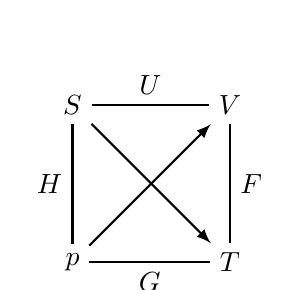
\begin{tikzpicture}
		\node(s)at(0,2){$S$};
		\node(v)at(2,2){$V$};
		\node(p)at(0,0){$p$};
		\node(t)at(2,0){$T$};
		\draw[thick](s)--(v)node[midway,above]{$U$};
		\draw[thick](s)--(p)node[midway,left]{$H$};
		\draw[thick](t)--(v)node[midway,right]{$F$};
		\draw[thick](t)--(p)node[midway,below]{$G$};
		\draw[thick,-latex](s)--(t);
		\draw[thick,-latex](p)--(v);
	\end{tikzpicture}
	\tikzchap Good physicists Have Studied Under Very Fine Teachers.
\end{center}
熵的标准全微分式:以$p,V,T$中两个为自变量,且将微分前系数用可测量表达出来的全微分式。比如以$T,V$
\[
	\d S=\kh{\pv ST}_V\d T+\kh{\pv SV}_T\d V=\frac{C_V}T\d T+\kh{\pv pT}_V\d V.
\]
\iffalse
\paragraph*{附:偏导关系式}
微积分II中我们学过:
\begin{align}
	 & 1.       & \kh{\pv XY}_Z & =\kh{\pv YX}_Z^{-1};                                             \\
	 & 2.       & \kh{\pv XY}_Z & =\dvd{\kh{\pv XW}_Z}{\kh{\pv YW}_Z};  \\
	 & 3.^\star & \kh{\pv XY}_Z & =-\dvd{\kh{\pv ZY}_X}{\kh{\pv ZX}_Y}; \\
	 & 4.       & \kh{\pv XY}_Z & =\kh{\pv XY}_W+\kh{\pv XW}_Y\kh{\pv WY}_Z.
\end{align}
% 可以用Jaccobi行列式证明。
\fi
利用偏导关系式
\begin{align*}
	\kh{\pv ST}_p=\kh{\pv ST}_V+\kh{\pv SV}_T\kh{\pv VT}_p,
\end{align*}
由Maxwell关系
\[
	\kh{\pv SV}_T=\kh{\pv pT}_V=-\dvd{\kh{\pv VT}_p}{\kh{\pv Vp}_T}.
\]
因此
\[
	C_p-C_V=-T\dvd{\kh{\pv VT}_p^2}{\kh{\pv Vp}_T}.
\]

\paragraph*{响应函数}定义体膨张系数
\begin{align}
	\alpha:=\frac1V\kh{\pv VT}_p.
\end{align}
等温压缩系数
\begin{align}
	\kappa_T:=-\frac1V\kh{\pv Vp}_T.
\end{align}
可得
\begin{align}
	C_p-C_V=\frac{VT\alpha^2}{\kappa_T}\geqslant 0.
\end{align}


\clearpage
\section{复相系统的热力学性质}
复相系统:由几个物理性质均匀的部分构成,每一个均匀部分称为一相。特别的,化学成分相同,但相不同构成单元复项系统。
\subsection{粒子数可变系统的热力学方程}
开放系统粒子数可变,设均匀系有$k$个组元,粒子数分别为$N_1,\ldots,N_k$;描述系统时,除几何、力学参量外,需加上化学参量。

以$T,p,\hkh{N_i}$为自变量,适用Gibbs自由能,$G$是广延量
\[
	G(T,p,\lambda\hkh{N_i})=\lambda G(T,p,\hkh{N_i}).
\]
由
\begin{theorem}{Euler定理}{Euler's Theorem}
	函数$f(x_1,\ldots,x_k)$是$m$阶齐次函数,若$\forall\lambda\leqslant 0$
	\[
		f(\lambda x_1,\ldots,\lambda x_k)=\lambda^mf(x_1,\ldots,x_k).
	\]
	在两边对$\lambda$求导,得到
	\[
		\sum_{i=1}^kx_i\pv f{x_i}=mf.
	\]
\end{theorem}
继而
\[
	G=\sum_{i=1}^kN_i\kh{\pv G{N_i}}_{\neq N_i}=:\sum_{i=1}^kN_i\mu_i.
\]
化学势$\mu_i$代表仅增加一个$i$组元粒子引起的$G$变化。摩尔Gibbs函数就是化学势$\mu$;孤立单元复相系,两相$\alpha$与$\beta$平衡的条件为化学势相同$\mu_\alpha=\mu_\beta$。
\paragraph*{化学反应}
考虑化学反应,设各化学计量数为$\nu_i$
\[
	0\rightleftharpoons\sum_{i=1}^r\nu_i{\mathrm A}_i.
\]
在恒温恒压的条件下,平衡时Gibbs自由能%\footnote{在混合系统中,总势一般不是各组分简单相加。}
最小
\begin{align}
	\d G=\sum_{i=1}^r\mu_i\d N_i=\d n\cdot\sum_{i=1}^r\nu_i\mu_i=0.
\end{align}
应当注意:$\mu_i$均来自于混合系统的Gibbs自由能。

非平衡时,由$\vd G<0$,可得$\textstyle\sum\nu_i\mu_i>0$时,$\d n<0$,平衡逆向进行。
\iffalse
考虑一个由理想气体参与的化学反应,理想气体的化学势
\[
	\mu_i=RT\ln p_i+\cns(T).
\]
带入上式可得,有
\[
	\sum_{i=1}^r\nu_iRT\ln p_i=\cns(T).
\]
%\[\prod p_i^{\nu_i}=-\exp\kh{\sum\nu_i\phi_i}.\]
又$p=RT\zkh{{\rm A}_i}$,%当$T$恒定时
\begin{align}
	\prod_{i=1}^r\zkh{{\rm A}_i}^{\nu_i}=:K(T).
\end{align}
%=(RT)^{-\sum\nu_i}\exp\kh{\sum\nu_i\phi_i}
$K$称为化学平衡常数,是$T$的函数。
\fi
\subsection{相变热力学}
前面已经提到,在有I和II两相共存的相变过程中,相变平衡的条件为$\mu_\mathrm I=\mu_\mathrm{II}$。

\paragraph*{Gibbs相律}有$n$个组分的系统在$r$个相共存时,系统$T,p,\mu_1,\ldots,\mu_n$共$(n+2)$个强度量,每个相有一个Gibbs-Duhem关系
\[
	S\d T-V\d p+\sum_{i=1}^nN_i\d\mu_i=0.
\]
因此自由度
\begin{align}
	f=n+2-r.
\end{align}
\paragraph*{Clapeyron方程}
同种物质两相共存时化学势相同
\begin{center}
	\begin{tikzpicture}
		\coor44Tp;
		\draw[thick,domain=1:3]plot(\x,{e^\x/7+.5});
		\node at(1.5,2.5){II};
		\node at(3,1){I};
	\end{tikzpicture}
	\tikzchap   I为高温相,II为低温相
\end{center}
共存曲线下,
\[
	\mu_\mathrm I(T,p)=\mu_\mathrm{II}(T,p).
\]
由$\d\mu=-s\d T+v\d p$
\iffalse
	故
	\[
		\pv{\mu_\mathrm I}T\d T+\pv{\mu_\mathrm I}p\d p=\pv{\mu_\mathrm{II}}T\d T+\pv{\mu_\mathrm{II}}p\d p.
	\]
	由Gibbs自由能给出Maxwell关系
	\begin{align*}
		\pw GTN=\pw GNT & \thus\kh{\pv\mu{T}}_N=-\kh{\pv SN}_T=-s, \\
		\pw GpN=\pw GNp & \thus\kh{\pv\mu{p}}_N=\kh{\pv VN}_p=v.
	\end{align*}
\fi
可得
\[
	\kh{s_\mathrm I-s_\mathrm{II}}\d T=\kh{v_\mathrm I-v_\mathrm{II}}\d p.
\]
由I相转变II相中需要吸收的相变潜热
\[
	\ell:=T(s_\mathrm I-s_\mathrm{II}).
\]
得到\begin{theorem}{Clapeyron方程}{Clapeyron equation}
	凝固点(或沸点)随压强的变化:
	\begin{equation}
		\dv Tp=\frac{T(v_\mathrm I-v_\mathrm{II})}\ell.
	\end{equation}
\end{theorem}
\begin{center}
	\begin{tikzpicture}
		\fill[gclr](0,0)--(2.06,1.28)--(4.31,2.4)--(4.31,3.36)--(4.9,3.36)--(4.9,0);
		\fill[sclr](0,0)--(2.06,1.28)--(1.08,3.36)--(0,3.36);
		\fill[lclr](2.06,1.28)--(1.08,3.36)--(4.31,3.36)--(4.31,2.4);
		%\shade[left color=lclr,right color=gclr](1.08,3.36) .. controls (1.14,2.83) and (1.44,1.95) .. (2.06,1.28)--(2.06,1.28) .. controls (3.03,1.44) and (3.71,1.84) .. (4.31,2.4)--(4.31,3.36);
		\draw[thick,fill=sclr](0,0) .. controls (0.76,0.09) and (1.56,0.58) .. (2.06,1.28) ;
		\draw[thick,fill=lclr](2.06,1.28) .. controls (3.03,1.44) and (3.71,1.84) .. (4.31,2.4) ;
		\draw[thick,fill=lclr](2.06,1.28) .. controls (1.44,1.95) and (1.14,2.83) .. (1.08,3.36) ;
		%\draw[dashed](2.06,1.28) .. controls (2.34,1.75) and (2.57,2.47) .. (2.64,3.35) ;
		\draw[dashed,thick](4.31,2.4)--(4.31,3.36);
		\draw[fill](2.06,1.28)circle(.05);
		\draw[fill](4.31,2.4)circle(.05);
		\coor{5.1}{3.6}Tp;
		\draw(2.06,0)node[below]{$T_\mathrm{tr}$}--(2.06,.1);
		\draw(4.31,0)node[below]{$T_\crt$}--(4.31,.1);
		\node at(.8,1.4){$\sfas$};
		\node at(3.1,.7){$\gfas$};
		\node at(2.6,2.6){$\lfas$};
	\end{tikzpicture}
	%\tikzchap 水的$T\vs p$图\\
	\begin{tikzpicture}
		\fill[gclr](0,0)--(2.06,1.28)--(4.31,2.4)--(4.31,3.36)--(4.9,3.36)--(4.9,0);
		\fill[sclr](0,0)--(2.06,1.28)--(2.64,3.35)--(0,3.36);
		\fill[lclr](2.06,1.28)--(2.64,3.36)--(4.31,3.36)--(4.31,2.4);
		\draw[thick,fill=sclr](0,0) .. controls (0.76,0.09) and (1.56,0.58) .. (2.06,1.28) ;
		\draw[thick,fill=lclr](2.06,1.28) .. controls (3.03,1.44) and (3.71,1.84) .. (4.31,2.4) ;
		%\draw[thick](2.06,1.28) .. controls (1.44,1.95) and (1.14,2.83) .. (1.08,3.36) ;
		\draw[thick,fill=sclr](2.06,1.28) .. controls (2.34,1.75) and (2.57,2.47) .. (2.64,3.36) ;
		\draw[dashed,thick](4.31,2.4)--(4.31,3.36);
		\draw[fill](2.06,1.28)circle(.05);
		\draw[fill](4.31,2.4)circle(.05);
		\coor{5.1}{3.6}Tp;
		\draw(2.06,0)node[below]{$T_\mathrm{tr}$}--(2.06,.1);
		\draw(4.31,0)node[below]{$T_\crt$}--(4.31,.1);
		\node at(1,1.8){$\sfas$};
		\node at(3.1,.7){$\gfas$};
		\node at(3.3,2.6){$\lfas$};
	\end{tikzpicture}
	\tikzchap 水(左)和一般纯净物(右)的$p\vs T$相图
\end{center}
对一般的汽-液相变,$v_\gfas\gg v_\lfas$,若气体符合理想气体,则有
\[
	\dv Tp\doteq\frac{Tv_\gfas}\ell=\frac{RT^2}{\ell p}\thus p=p_0\exp\fkh{\frac\ell{R}\kh{\frac1{T_0}-\frac1T}}.
\]
水凝固存在反常膨胀,$\d T/\d p<0.$
\paragraph*{气液两相的转变和临界点}
考虑等温线
\begin{center}
	\begin{tikzpicture}
		\fill[lclr](0,0)--(0,5.13)--(1.42,5.13)--(2.09,3.98)--(0.91,0);
		\fill[gclr](1.42,5.13)--(2.09,3.98)--(3,.35)--(5.79,.35)--(5.79,5.13);
		\fill[glclr](0.91,0)--(0.91,.49)--(5.35,.49)--(5.79,0.35)--(5.79,0);
		\draw[dashed,fill=glclr](0.91,0.49) .. controls (0.93,1.72) and (1.27,3.98) .. (2.09,3.98) .. controls (2.91,3.98) and (4.11,1.01) .. (5.35,0.49) ;
		\draw[thick](0.65,5.13) -- (1.13,2.47) -- (3.54,2.47) ;
		\draw[thick](3.54,2.47) .. controls (4.24,1.72) and (4.89,1.4) .. (5.79,1.25) ;
		\draw[thick](1.03,5.13) -- (1.37,3.24) -- (2.99,3.24) ;
		\draw[thick](2.99,3.24) .. controls (3.9,2.4) and (4.82,2.11) .. (5.79,2.08)node[right]{$T<T_\crt$};
		\draw[thick,fill=gclr](1.42,5.13) .. controls (1.49,4.73) and (1.68,3.99) .. (2.09,3.98) .. controls (2.5,3.97) and (4.64,2.88) .. (5.79,2.91)node[right]{$T=T_\crt$};
		\draw[thick](1.8,5.13) .. controls (2.11,4.24) and (3.43,3.97) .. (5.79,3.74)node[right]{$T>T_\crt$};
		%\node[right]at(5.79,4.57){$T\gg T_\crt$};
		\coor6{5.5}Vp;
		\draw[fill](2.09,3.98)circle(.05)node[above]{C};
		\node at(.5,2.5){$\lfas$};
		\node at(2.5,1.2){$\lfas+\gfas$};
		\node at(4,4.5){$\gfas$};
	\end{tikzpicture}
	\tikzchap $p\vs V$相图,等温线
\end{center}
当$T<T_\crt$时,会存在气液共存区,在共存区中化学势相同
\[
	\mu_\lfas(T,p)=\mu_\gfas(T,p).
\]
由于图中是等温线,所以共存区中等温线垂直于$p$轴;在临界点C有
\begin{align}
	\pv pV=0,\qquad\pv[2]pV=0.
\end{align}
理想气体不存在液化,下面考虑Van der Waals气体。
\begin{example}{Van der Waals气体的约化变量}{Reduced Variables of Van der Waals Gas}
	对于临界温度$T_\crt$
	\begin{align}
		\begin{cases}
			\pv pv=-\frac{RT}{(v-b)^2}+\frac{2a}{v^3}=0, \\
			\pv[2]pv=\frac{2RT}{(v-b)^3}-\frac{6a}{v^4}=0.
		\end{cases}\thus\begin{cases}
			v_\crt=3b,              \\
			T_\crt=\frac{8a}{27Rb}.
		\end{cases}.
	\end{align}
	此时
	\begin{align}
		p_\crt=\frac{RT_\crt}{v_\crt-b}-\frac a{v_\crt^2}=\frac a{27b^2}.
	\end{align}
	可以定义约化变量$\tilde T:=T/T_\crt$等,可得
	% \[\tilde p=\frac{8\tilde T}{3\tilde v-1}-\frac3{\tilde v^2}.\]
	\begin{align}
		\kh{\tilde p+\frac3{\tilde v^2}}\kh{\tilde v-\frac13}=\frac83\tilde T.
	\end{align}
\end{example}
气液共存线上气液摩尔比$x$,则
\[
	v=v_\gfas x+v_\lfas(1-x),\thus x=\frac{v-v_\lfas}{v_\gfas-v_\lfas}.
\]
\begin{center}
	\begin{tikzpicture}[scale=.8]
		\draw[dashed,glclr](0.91,0.49) .. controls (0.93,1.72) and (1.27,3.98) .. (2.09,3.98) .. controls (2.91,3.98) and (4.11,1.01) .. (5.35,0.49) ;
		\draw[thick](0.65,5.13) -- (1.13,2.47)node[midway,left]{$\lfas$} -- (3.54,2.47)node[midway,above]{$\lfas+\gfas$};
		\draw[thick](3.54,2.47) .. controls (4.24,1.72) and (4.89,1.4) .. (5.79,1.25)node[midway,above]{$\gfas$};
		\coor6{5.5}vp;
		\draw[dashed](1.13,2.47)--(1.13,0)node[below]{$v_\lfas$};
		\draw[dashed](2,2.47)--(2,0)node[below]{$v$};
		\draw[dashed](3.54,2.47)--(3.54,0)node[below]{$v_\gfas$};
	\end{tikzpicture}
	\tikzchap 杠杆原理
\end{center}

投影到$T\vs V$图上与$p\vs V$图类似,只有$p<p_\crt$时才会有气液共存区,共存区的等压线垂直于$T$轴(对应沸点)。
\subsection{Landau相变理论}
在超导、磁性等一大类相变中,有一区别不同相的热力学量,称为序参量$\eta$。

无序相序参量$\eta=0$;有序相$\eta\neq 0$,对应对称破缺;$\eta$可以是复数(超导、超流);序参量有一维标量,也可以是二维和三维的。可以与
空间的维数不同。

相变中,Gibbs自由能
\[
	\d G=-S\d T-y\d Y+\sum\mu_i\d N_i=0.
\]
对于固定$Y,T$下实现的过程有$\mu_i$必须相等,但对导数$S,y$无限制。若$S,y$在相变点不连续,则称相变为一级相变;若二阶导数不连续,则称为二级相变。

临界点:连续相变的相变点,临界温度$T_\crt$;临界现象:物质在连续相变临界点邻域的统计热力学行为。

唯象的,Landau自由能在临界点
\begin{align}
	F(T,\eta)=F_0(T)+\frac12a(T)\eta^2+\frac14b(T)\eta^4+\cdots,
\end{align}
由于系统对$\pm\eta$是对称的,展开中不含$\eta$的奇次幂。

求极值
\[
	\pv F\eta=\eta(a+b\eta^2)=0,\quad\pv[2]F\eta=a+3b\eta^2>0.
\]
有三个解
\[
	\eta=0,\pm\sqrt{-\frac ab}.
\]
$\eta=0$对应无序态,$T>T_\crt$;$\eta_\pm$对应有序态,$T<T_\crt$。当$T\to T_\crt$时,序参量$\eta$在$T_\crt$连续地由零转变到非零,即$a(T_\crt)=0$。

$T_\crt$附近泰勒展开
\[
	a(T)=a_0\kh{\frac T{T_\crt}-1},\quad b(T)=b_0.
\]
$T<T_\crt$时,$a(T)<0$,故$b_0>0$。
\[
	\eta=
	\begin{cases}
		0,&T\geqslant T_\crt\\
		\pm\sqrt{\frac{a_0}{b_0}\kh{1-\frac T{T_\crt}}},&T<T_\crt
	\end{cases}
\]
临界指数$\beta=1/2$。

熵是连续的
\begin{align*}
	S=-\pv FT=S_0-\frac{a_0}{2T_\crt}\eta^2=
	\begin{cases}
		S_0,                             & T\geqslant T_\crt \\
		S_0+\frac{a_0^2}{2b_0T_\crt}\kh{\frac T{T_\crt}-1}, & T<T_\crt
	\end{cases}
	\rqed
\end{align*}
比热却不连续了,
\begin{align*}
	C=T\pv ST=
	\begin{cases}
		C_0,                 & T\geqslant T_\crt \\
		C_0+\frac{a_0^2}{2b_0T_\crt^2}T, & T<T_\crt
	\end{cases}
	\rqed
\end{align*}
因此是\textbf{二级相变}。有序相的比热大于无序相的比热,且$T=T_\crt$处比热的突变是有限的,$\alpha=\alpha'=1$。
\subparagraph*{外加场$B$}在弱场$B$下,序参量$m$
\[
	G(m,B)=F_0+\frac12am^2+\frac14bm^2-Bm.
\]
平衡时
\[
	\pv Gm=a\eta+bm^3-B=0.
\]
$T=T_\crt$时,$a=0,\;B=bm^3$故$\delta=3$。

磁化率
\[
	\chi=\mu_0\kh{\pv mB}_T=\frac{\mu_0}{a+3bm^3}=
	\begin{cases}
		\frac{\mu_0}{a_0}\kh{\frac T{T_\crt}-1}^{-1},&T\geqslant T_\crt \\
		\frac{\mu_0}{2a_0}\kh{\frac T{T_\crt}-1}^{-1}, & T<T_\crt
	\end{cases}
\]
$\gamma'=\gamma=1$。

临界指数$\alpha=1,\,\beta=1/2,\,\gamma=1,\,\delta=3$与实验结果有差异,原因是没考虑涨落。

\clearpage
\part{统计物理}
统计物理是将宏观性质看作是对应微观量的统计平均的微观理论。单粒子的力学规律是决定论的,如量子力学的Schrödinger方程、经典力学中的正则方程或Newton II;而宏观系统的统计规律是非决定论的,用宏观量指定的宏观状态对应大量不同的微观状态.
\section{近独立粒子系统的统计分布}
概率基本知识:概念、互斥事件几率的加法定理、独立事件几率的乘法定理、条件概率、多个随机变量的联合概率分布、统计平均值和涨落等。
\begin{definition}{二项分布}{Binominal Distribution}
	$N$次独立重复实验中事件发生$n$次概率
	\[
		P_N(n)=\binom Nnp^nq^{N-n}=\frac{N!}{n!(N-n)!}p^nq^{N-n}.
	\]
	其中$p$为事件发生的概率,$q=1-p.$
\end{definition}
\begin{definition}{Possion分布}{Possion Distribution}
	当二项分布的$N\gg 1,p\ll 1$时,可近似为Possion分布
	\[
	P(n)=\e{-\avg n}\frac{\avg n^n}{n!}.
	\]
	Possion分布的期望和标准差均为$\avg n.$
\end{definition}
\begin{definition}{Gauss分布}{Gauss Distribution}
	当二项分布的$N\gg 1,p\doteq q$时,可约化为Gauss分布
	\[
		P(n)=\frac1{\sqrt{2\pi\sigma^2}}\e{-(n-\avg n)^2/2\sigma^2}.
	\]
	对应Gauss积分
	\[
	\int\iti\e{-x^2}\d x=\sqrt\pi.
\]
\end{definition}
\subsection{近独立粒子系统}
所谓近独立粒子,就是在平均意义下
\begin{center}
	$0<$粒子间作用能$\ll$单个粒子能量
\end{center}
对于单粒子状态可以通过\textbf{Schrödinger方程}
\[
	\hat H\ket n=\varepsilon_n\ket n.
\]
解得能量本征值$\varepsilon_n$,简并度$\omega_n$和量子态$\ket n$。
\begin{example}{一维无穷深势阱}{1-D Infinte Square Potential Well}
	一维无穷深势阱能量本征值和简并度
	\[
	\varepsilon_n=\frac{n^2h^2}{8mL^2},\quad\omega_n=1\quad n=1,2,\ldots.
\]
	能级间能量差
	\[
	\D\varepsilon=\kh{2n+1}\frac{h^2}{8mL^2}\sim\SI{e-36}\joule.
\]
	远小于热运动能量($\kB T$),因此能量准连续.
\end{example}
粒子按量子态的一个分配方式,称为系统的一个微观状态;粒子按能级的一个分布称为系统的一个宏观状态.
分布与自旋有关,分布与微观状态不同,一组分布对应大量不同微观状态.
记$\hkh{a_i}$表示$a_i$个粒子处于能级$\varepsilon_i.$
\begin{definition}{Boltzmann系统}{Boltzmann System}
	定域系统如:固体晶格.粒子可以分辨,量子态容纳粒子数不受限制.

	$N$粒子全排除去各能级内全排;$a_i$可占据$\omega_i$中任一态
	\begin{align}
		\Om=\frac{N!}{\prod a_i!}\prod\omega_i^{a_i}=N!\prod\frac{\omega_i^{a_i}}{a_i!}.
	\end{align}
\end{definition}

\begin{definition}{Bose系统}{Bose System}
	Bose子:自旋量子数整数.不可分辨,量子态容纳粒子数不受限制.

	从$a_i+\omega_i$个粒子和空位的间隔中插$a_i$个隔板
	\begin{align}
		\Om[B]=\prod\binom{a_i+\omega_i-1}{a_i}=\prod\frac{\kh{a_i+\omega_i-1}!}{a_i!\kh{\omega_i-1}!}.
	\end{align}
\end{definition}
\begin{definition}{Fermi系统}{Fermi System}
	Fermi子:自旋量子数半整数.不可分辨,量子态容纳最多一个粒子.(Pauli不相容原理)

	从$\omega_i$中挑出$a_i$个粒子位
	\begin{align}
		\Om[F]=\prod\binom{\omega_i}{a_i}=\prod\frac{\omega_i!}{a_i!\kh{\omega_i-a_i}!}.
	\end{align}
\end{definition}
\begin{theorem}{统计物理平衡态假设}{Equilibrium Hypothesis}
	\textbf{等几率假设}(Planck):分布$\hkh{a_i}$的热力学几率$\propto\Omega_i\hkh{a_i}.$

	\textbf{最可几分布}:将热力学几率最大的分布近似作为平衡态分布.
\end{theorem}
% 孤立系统$N,V,E$确定
\paragraph{Bose分布}
$a_i\gg 1,\omega_i\gg 1$由Stirling公式
\[
	\ln x!\doteq x\kh{\ln x-1}\,{\color{lightgray}+\ln\sqrt{2\pi x},}\quad x\gg 1.
\]
可约化Bose分布
\begin{align*}
	\ln\Om[B]\doteq\sum\fkh{a_i\ln\kh{1+\frac{\omega_i}{a_i}}+\omega_i\ln\kh{1+\frac{a_i}{\omega_i}}}.
\end{align*}

再结合定解条件
\[
	N=\sum a_i,\quad E=\sum a_i\varepsilon_i.
\]
利用Lagrange待定乘子法
\begin{gather*}
	\pp{a_i}\ln\Om[B]+\alpha\cdot\pp{a_i}\kh{N-\sum a_i}+\beta\cdot\pp{a_i}\kh{E-\sum a_i\varepsilon_i}=0\\
	\ln\kh{1+\frac{\omega_i}{a_i}}-\alpha-\beta\ve_i=0.
\end{gather*}
解得
\begin{align}
	a_i=\frac{\omega_i}{\e{\alpha+\beta\varepsilon_i}-1}.
\end{align}
% Bose-Einstein分布(简称Bose分布)

检验该点为极大值点
\[
	\pp[2]{a_i}\Om[B]=-\frac{\omega_i/a_i}{\omega_i+a_i}<0.
\]
\paragraph{Fermi分布}
$a_i\gg 1,\omega_i\gg a_i$,类似Bose分布
\begin{gather}\notag
	\ln\Om[F]\doteq\sum\fkh{a_i\ln\kh{\frac{\omega_i}{a_i}-1}-\omega_i\ln\kh{1-\frac{a_i}{\omega_i}}}.\\
	% Lagrange待定乘子法
	a_i=\frac{\omega_i}{\e{\alpha+\beta\varepsilon_i}+1}.
\end{gather}

% Fermi-Dirac分布(简称Fermi分布)

检验该点为极大值点
\[
	\pp[2]{a_i}\Om[F]=-\frac{\omega_i/a_i}{\omega_i-a_i}<0.
\]
\paragraph*{半经典分布}
% 若取基态能量为0,则$\varepsilon_i\geqslant 0$,
当$\e\alpha\gg 1$,Bose分布和Fermi分布变为
\begin{align}
	a_i=\omega_i\e{-\alpha-\beta\varepsilon_i}.
\end{align}
因此要求$a_i\ll\omega_i$(非简并)
\begin{align}
	\Om[S]=\prod\frac{\omega_i^{a_i}}{a_i!}.
\end{align}
与Boltzmann分布相比,$N!$仅是系数差别,不影响求最可几分布.
\paragraph*{最可几方法误差估计}
在最可几分布$a_\mathrm m$处展开
\begin{align*}
	\ln\Om & =\ln\Omm+0+\frac12\sum_i\underline{\pn 2{a_i}\Omm}\,\delta a_i^2+\cdots
	% \ln\Omega\hkh{a_i} & =\ln\Omega\hkh{a_{i\mathrm m}}+\sum_i\pv{\Omega}{a_i}\hkh{a_{i\mathrm m}}(a_i-a_{i\mathrm m})+\frac12\sum_i\spd{\Omega}{a_i}\hkh{a_{i\mathrm m}}(a_i-a_{i\mathrm m})^2+\cdots
\end{align*}
因此
\[
	\ln\frac\Om\Omm\doteq-\frac12\sum_i\frac{\delta a_i^2}{a_\mathrm m}.
\]
若$\dvd{\delta a_i}{a_\mathrm m}\sim 10^{-4},$
\[
	\frac\Om\Omm\sim\e{-10^{23-8}}\lll 1.
\]
\subsection{宏观量的统计表达式}
\begin{definition}{配分函数}{Partition Function}
	定义配分函数
	\begin{align}
		Z(\beta,y):=\sum_i\omega_i\e{-\beta\varepsilon_i}.
	\end{align}
	其中$y$是外参量,单粒子能级$\varepsilon_i$是$y$的函数.
\end{definition}
半经典分布中,分子数
\[
	N=\sum_ia_i=\sum_i\omega_i\e{-\alpha-\beta\varepsilon_i}=Z\e{-\alpha},
\]
用配分函数$Z$表示$\alpha$
\begin{align}
	\spark{\alpha=\ln\frac ZN.}
\end{align}
内能
\[
	E=\sum_ia_i\varepsilon_i=\sum_i\varepsilon_i\omega_i\e{-\alpha-\beta\varepsilon_i}=-\e{-\alpha}\pv Z\beta=-\frac NZ\pv Z\beta.
\]
即
\begin{align}
	\spark{E=-N\pv{\ln Z}\beta.}
\end{align}

准静态过程中,
\[
	\d E\equiv\sum a_i\d\varepsilon_i+\varepsilon_i\d a_i=\delta W+\delta Q.
\]

功
\[
	\delta W=\sum_iY_k\d y_k
\]
其中$Y_k,y_k$分别是广义力和广义坐标(如$-p,V$).
\[
	\sum_kY_k\d y_k=\sum_ia_i\d\varepsilon_i=\sum_i a_i\sum_k\pv{\varepsilon_i}{y_k}\d y_k,
\]
故
\[
	Y_k=\sum_ia_i\pv{\varepsilon_i}{y_k}=\sum_i\omega_i\e{-\alpha-\beta\varepsilon_i}\pv{\varepsilon_i}{y_k}.
\]
物态方程
\begin{align}
	\spark{Y_k=-\frac N\beta\pv{\ln Z}{y_k}.}
\end{align}

热
\[
	\delta Q=\d E-\sum_ia_i\d\varepsilon_i=-N\d\kh{\pv{\ln Z}\beta}+\frac N\beta\sum_k\pv{\ln Z}{y_k}\d y_k.
\]
又
\[
	\d\kh{\ln Z}=\pv{\ln Z}\beta\d\beta+\sum_k\pv{\ln Z}{y_k}\d y_k.
\]
故
\begin{align*}
	T\d S & =-N\d\kh{\pv{\ln Z}\beta}+\frac N\beta\kh{\d\kh{\ln Z}-\pv{\ln Z}\beta\d\beta} \\
	      & =\frac N\beta\d\kh{\ln Z-\beta\pv{\ln Z}\beta}.
\end{align*}
% 因此
% \[\d S=\frac N{\beta T}\d\kh{\ln Z-\beta\pv{\ln Z}\beta}.\]
两边全微分,要求系数为常数,定义Boltzmann常数
\[
	\frac1{\beta T}=:\kB=\SI{1.380649e-23}{\J\per\K}.
\]
故
\begin{align}
	\spark{S-S'=N\kB\kh{\ln Z-\beta\pv{\ln Z}\beta}.}
\end{align}
\begin{theorem}{Boltzmann关系}{Boltzmann Relation}
	熵
	\begin{align}
		S=\kB\ln\Om.
	\end{align}
	其中$\kB$为Boltzmann常数.
\end{theorem}
通过Boltzmann关系可以确定熵,粒子不可分辨的半经典分布中
\begin{align}\notag
	S & =\kB\sum\ln\zkh{a_i\ln\omega_i-a_i\kh{\ln a_i-1}}=\kB\sum\ln a_i\kh{\alpha+\beta\varepsilon_i+1} \\\notag
	  & =\kB\kh{N\alpha+\beta E+N}=\kB\kh{N\ln\frac ZN-N\beta\pv{\ln Z}N+N}                              \\
	  & =N\kB\kh{\ln Z-\beta\pv{\ln Z}\beta-\ln N+1}.
\end{align}
和之前的结果比较可以确定$S'$
\[
	S'=N\kB\kh{1-\ln N}\doteq-\kB\ln N!.
\]
对应的,粒子可分辨的Boltzmann分布$S'=0.$

其他宏观量也可以表示,自由能
\begin{align}
	F=E-TS=-N\kB T\ln Z-TS'.
\end{align}
化学势在半经典分布中
\[
	\mu=\kh{\pv FN}_T=-\alpha\kB T.
\]
Boltzmann分布$\mu=-\kB T\ln Z$。
\subsection{单粒子态的半经典描述}
定义系统的Hamilton量$H\equiv\varepsilon$,则广义坐标$q_i$与广义动量$p_i$有关系
\[
	\dot q_i=\pv H{p_i},\quad\dot p_i=-\pv H{q_i}.
\]
\begin{definition}{$\mu$空间}{Mu Space}
	$\mu$空间是粒子的广义坐标$q_i$与广义动量$p_i$所张的空间.相体积元
	\begin{align}
		\d\omega=\prod_{i=1}^\gamma\d q_i\nd p_i.
	\end{align}
	其中$\gamma$为粒子自由度.
\end{definition}
单粒子能量看成$q,p$的连续函数;由不确定性关系$\D q\D p=h$
\begin{theorem}{极限定理}{Limit Theorem}
	大量子数的状态在$\mu$空间对应$h^\gamma$相体积。
\end{theorem}
每个状态上的粒子数
\begin{align}
	\frac{a_i}{\omega_i}=\e{-\alpha-\beta\varepsilon}.
\end{align}
因此$\d\omega$内所含的粒子数
\[
	h^{-\gamma}\d\omega\cdot\e{-\alpha-\beta\varepsilon}.
\]
% 因此 % 😅 二次元能不能死一死
% \[N=h^{-\gamma}\int\e{-\alpha-\beta\varepsilon}\d\omega=\e{-\alpha}Z.\]
又$N=\e{-\alpha}Z$,故
\begin{align}
	Z(\beta,y)=h^{-\gamma}\int\e{-\beta\varepsilon}\d\omega.
\end{align}
而能量在$\kh{\varepsilon,\varepsilon+\d\varepsilon}$上的粒子数
\[
	n(\varepsilon)\d\varepsilon=g(\varepsilon)\e{-\alpha-\beta\varepsilon}\d\varepsilon.
\]
比较可得态密度
\[
	g(\varepsilon)=h^{-\gamma}\dv{\Omega(\varepsilon)}\varepsilon.
\]
其中$\Omega(\varepsilon)$表示能量$\varepsilon$曲面所围相体积。这样
\begin{align}
	Z(\beta,y)=\int\zti g(\varepsilon)\e{-\beta\varepsilon}\d\varepsilon.
\end{align}
\newpage
\subsection*{验证极限定理}
\begin{example}{谐振子}{Harmonic Oscillator}
	一维谐振子,Hamilton量
	\[
		\varepsilon=\frac{p^2}{2m}+\frac12m\omega^2x^2.
	\]
	因此
	\[
		\Omega(\varepsilon)=\pi\sqrt{2m\varepsilon}\sqrt{\frac{2\varepsilon}{m\omega^2}}=\frac{2\pi\varepsilon}\omega.
	\]
	\[
		g(\varepsilon)=\frac1h\dv\Omega\varepsilon=\frac{2\pi}{h\omega}.
	\]
	另一方面
	\[
		\varepsilon_n=\kh{n+\frac12}\hbar\omega,\quad\omega_n=1.
	\]
	相体积为$h$
	\[
		\D\Omega(\varepsilon_n)=\frac{2\pi}\omega\hbar\omega=h.
	\]
	\tcblower
	二维谐振子,Hamilton量
	\[
		\varepsilon=\frac{p_x^2+p_y^2}{2m}+\frac12m\omega^2\kh{x^2+y^2}.
	\]
	借助4维单位球体积公式
	\[
		\Omega(\varepsilon)=\frac{\pi^2}2\cdot2m\varepsilon\frac{2\varepsilon}{m\omega^2}=\frac{2\pi^2\varepsilon^2}{\omega^2}.
	\]
	\[
		g(\varepsilon)=\frac1{h^2 }\dv\Omega\varepsilon=\frac{4\pi^2\varepsilon}{h^2\omega^2}.
	\]
	另一方面
	\[
		\varepsilon_n=\kh{n+1}\hbar\omega,\quad\omega_n=n+1.
	\]
	相体积为
	\[
		\frac{\D\Omega(\varepsilon_n)}{n+1}=\frac{2\pi^2\hbar^2\kh{2n+1}}{n+1}\to h^2.
	\]
\end{example}
\begin{example}{转子}{Rotor}
	系统的转动惯量$I$,则Hamilton量
	\[
		\varepsilon=\frac1{2I}\kh{p_\theta^2+\frac1{\sin^2\theta}p_\phi^2}.
	\]
	因此
	\begin{gather}\notag
		\Omega(\varepsilon)=\int\d\theta\nd\phi\int\d p_\theta\nd p_\phi=2\pi\int_0^\pi\pi\sqrt{2I\varepsilon}\sqrt{2I\varepsilon\sin^2\theta}\d\theta=8\pi^2I\varepsilon;\\
		g(\varepsilon)=\frac1{h^2}\dv\Omega\varepsilon=\frac{8\pi^2I}{h^2}.
	\end{gather}
	另一方面
	\[
		\varepsilon_\ell=\frac{\hbar^2}{2I}\ell(\ell+1),\quad\omega_\ell=2\ell+1.
	\]
	相体积为
	\[
		\frac{\D\Omega(\varepsilon_n)}{2\ell+1}=\frac{8\pi^2\hbar^2\ell}{2\ell+1}\to h^2.
	\]
\end{example}
\begin{example}{单原子分子}{Monatomic Molecule}
	Hamilton量
	\[
		\varepsilon=\frac1{2m}\kh{p_x^2+p_y^2+p_z^2}.
	\]
	在体积为$V$的容器中,
	\begin{gather}\notag
		\Omega(\varepsilon)=V\int_0^{\sqrt{2m\varepsilon}}4\pi p^2\d p=\frac{4\pi V}3\kh{2m\varepsilon}^{3/2};\\
		g(\varepsilon)=\frac1{h^3}\dv\Omega\varepsilon=\frac{2\pi V}{h^3}\kh{2m}^{3/2}\sqrt\varepsilon.
	\end{gather}
	若考虑自旋,还应乘自旋因子$g_s=2s+1$。

	另一方面
	\[
		\varepsilon_n=\frac{h^2}{8mL^2}\kh{n_x^2+n_y^2+n_z^2},\quad n=\set{n_x,n_y,n_z}{n_i=1,2,\ldots}
	\]
	简并度$\omega_n$近似为
	\[
		G(\ve)=\frac18\cdot\frac{4\pi}3\kh{\frac{8mL^2\varepsilon}{h^2}}^{3/2}=\frac{4\pi}{3}\kh{2\pi\varepsilon}^{3/2}Vh^{-3}.
	\]
	因此每个状态的相体积
	\[
		\frac{\Omega(\varepsilon)}{G(\varepsilon)}=h^3.
	\]
	\tcblower
	极端相对论情形下
	\[
		\varepsilon=cp=c\sqrt{p_x^2+p_y^2+p_z^2}.
	\]
	故
	\begin{align}
		\Omega(\varepsilon)=V\cdot\frac{4\pi}3\kh{\frac\varepsilon{c}}^3,\quad g(\varepsilon)=\frac{4\pi V}{h^3c^3}\varepsilon^2.
	\end{align}
\end{example}
由例 \ref{exm:Monatomic Molecule} 可知,非相对论情形下
\[
	\varepsilon=\frac1{2m}\kh{\frac h{2L}}^2\kh{n_x^2+n_y^2+n_z^2}=\frac{h^2}{8m}\kh{n_x^2+n_y^2+n_z^2}V^{-2/3}.
\]
故
\[
	\pv\varepsilon V=\frac{h^2}{8m}\kh{n_x^2+n_y^2+n_z^2}\kh{-\frac23}V^{-5/3}=-\frac23\frac\varepsilon V.
\]
压强
\begin{align}
	p=-\sum a_i\pv{\varepsilon_i}V=\frac23\sum a_i\frac{\varepsilon_i}V=\frac23\frac UV.
\end{align}

而极端相对论情形下
\[
	\varepsilon=c\cdot\frac h{2V^{1/3}}\sqrt{n_x^2+n_y^2+n_z^2}.
\]
相似的
\begin{align}
	p=\frac13\frac UV.
\end{align}
\clearpage
\section{Boltzmann分布}
\subsection{理想气体}
理想气体在常温常压下满足非简并条件
\[
	\e\alpha\gg 1.
\]
符合半经典分布.分子运动可分为质心平动和内部运动,两种运动独立
\[
	\varepsilon\tot=\varepsilon_\tl+\varepsilon_\i,\quad\omega\tot=\omega_\tl\omega_\i.
\]
\subsubsection*{质心平动}
$\varepsilon_\tl$准连续
\[
	\varepsilon_\tl=\frac1{2m}\kh{p_x^2+p_y^2+p_z^2}.
\]
由例~\ref{exm:Monatomic Molecule},配分函数
\begin{align}\notag
	Z_\tl(\beta,V) & =\int\zti g(\varepsilon)\e{-\beta\varepsilon}\d\varepsilon                                                                      \\
	               & =\frac{2\pi V}{h^3}\kh{2m}^{3/2}\int\zti\sqrt\varepsilon\e{-\beta\varepsilon}\d\varepsilon=V\kh{\frac{2\pi m}{h^2\beta}}^{3/2}.
\end{align}

单原子分子只有质心平动
\[
	N=\e{-\alpha}Z_\tl,\thus\e{\alpha}=\frac VN\kh{\frac{2\pi m\kB T}{h^2}}^{3/2}\gg 1.
\]
说明稀薄、高温、质量大的情况下和非简并条件符合得很好.
\begin{gather}
	E_\tl=-N\pv{\ln Z_\tl}\beta=\frac32N\kB T.\\
	C_V^\tl=\kh{\pv ET}_V=\frac32N\kB.
\end{gather}
物态方程
\begin{align}
	p=\frac N\beta\pv{\ln Z_\tl}V=\frac{N\kB T}V.
\end{align}
熵
\begin{align}\notag
	S_\tl & =N\kB\kh{\ln Z_\tl-\beta\pv{\ln Z_\tl}\beta-\ln N+1}                 \\
	      & =\frac52N\kB+N\kB\ln\fkh{\frac VN\kh{\frac{2\pi m\kB T}{h^2}}^{3/2}}
\end{align}
\subsubsection*{振动}
考虑一维振动,取约化质量$\mu$,有
\[
	\varepsilon_\vb(n)=h\nu\kh{n+\frac12},\quad\omega_\vb(n)=1.
\]
能量间距
\[
	\D\varepsilon_\vb=h\nu\sim\SI{0.1}\electronvolt.
\]
远大于室温下$\kB T\sim\SI{0.025}\electronvolt.$因此必须考虑能级的分立性.

定义振动的特征温度
\[
	\theta_\vb:=\frac{\D\varepsilon_\vb}\kB=\frac{h\nu}\kB\sim\SI{e3}\K.
\]
则配分函数
% \[Z_\nu=\sum\omega_\nu(n)\e{-\beta\varepsilon_\nu(n)}.\]
\begin{align}
	Z_\vb=\sum\fmto n0\e{-(n+1/2)\beta h\nu}=\frac{\e{-\theta_\vb/2T}}{1-\e{-\theta_\vb/T}}=\frac12\csch\kh{\frac{\theta_\vb}{2T}}.
\end{align}
振动内能
\begin{align}
	E_\vb=-N\pv{\ln Z_\vb}\beta=Nh\nu\fkh{\frac12+\underset{\text{激发能}}{\frac{\e{-\beta h\nu}}{1-\e{-\beta h\nu}}}}=:N\avg\varepsilon.
\end{align}
其中$\avg\varepsilon$为单个原子的振动能。

比热
\begin{align}
	C_V^\vb=\kh{\pv{E_\vb}T}_V=N\kB\Einst\!\kh{\frac{\theta_\vb}T},
\end{align}
其中Einstein函数
\[
	\Einst(x):=\frac{x^2\e x}{\kh{\e x-1}^2}.
\]

低温极限,由
\[
	x\gg 1,\quad\Einst(x)\doteq x^2\e{-x}\ll 1
\]
因此比热
\begin{align}
	C_V^\vb\doteq N\kB\kh{\frac{\theta_\vb}T}^2\e{-\theta_\vb/T}.
\end{align}
相对振动而言,常温属于低温范围,故振动自由度对$C_V$贡献很小。

高温极限,能量准连续
\begin{align*}
	Z_\vb & =\int\zti g(\ve)\e{-\beta\ve}\d\ve=\frac{2\pi}{h\omega}\int\zti\e{-\beta\ve}\d\ve=\frac{2\pi}{\beta h\omega}=\frac T{\theta_\vb}.
\end{align*}
内能
\[
	E_\vb=N\kB T.
\]

或由低温算得的结果,使$\beta\to0$
\[
	E_\vb\doteq Nh\nu\kh{\frac12+\frac1{\beta h\nu}}\doteq N\kB T.
\]
这里比较有三个自由度$p_x,p_y,p_z$的平动能量$E_\tl=3\kB T/2$和有两个自由度的振动能量$E_\vb=\kB T$,可以总结这样一个规律:
\begin{theorem}{能量均分定理}{Equi-Partition Theorem}
	高温下,能量准连续,能量的每个自由度对能量贡献为$\kB T/2$。
\end{theorem}
\subsubsection*{转动}
以异核双原子分子为例,\footnote{同核需考虑全同性原理。比如正氢:两个氢核自旋平行,$\ell$为奇数;仲氢:两个氢核自旋反平行,$\ell$为偶数。}
\[
	\varepsilon_\rt(\ell)=\frac{\hbar^2}{2I}\ell(\ell+1),\quad\omega_\rt(\ell)=2\ell+1.
\]

转动特征温度
\[
	\ct_\rt=\frac{\hbar^2}{2I\kB}\sim\SI{10}\K.
\]
配分函数
\[
	Z_\rt=\sum\fmto{\ell}0(2\ell+1)\e{-\ell(\ell+1)\,\theta_\rt/T}.
\]
并没有显式表达式。

高温极限下,能量准连续
\[
	Z_\rt=\int\zti g(\ve)\e{-\beta\ve}\d\ve=\frac{8\pi^2I}{h^2}\cdot\frac1\beta=\frac T{\theta_\rt}.
\]
或由$\ct_\rt/T\ll 1$
\[
	Z_\rt\doteq\int_0^{+\infty}\e{-\ell(\ell+1)\,\theta_\rt/T}\cdot(2\ell+1)\d\ell=\frac T{\ct_\rt}.
\]
能量和比热
\begin{align}
	E_\rt=N\kB T,\quad C_V^\rt=N\kB.
\end{align}

低温极限,$\ct_\rt/T\gg 1$,$Z_\rt$的项很快趋于0
\[
	Z_\rt=1+3\e{-2\ct_\rt/T},
\]
能量和比热
\begin{align}
	E_\rt&=6N\kB\ct_\rt\e{-2\ct_\rt/T},\\
	C_V^\rt&=12N\kB\kh{\frac{\ct_\rt}T}^2\e{-2\ct_\rt/T}.
\end{align}

原子内部结构:电子、原子核等的自由度对宏观量(特别是$C_V$)无贡献。因为在稳定性、结合能、能级间距上,从分子、原子到原子核越来越稳定,特征温度越来越高,越来越难以被激发。即,结合的紧密的自由能被冻结了,通常不激发。
\subsectionstar{Maxwell速度分布律}
考虑气体分子质心平动
\[
	\varepsilon=\frac1{2m}\kh{p_x^2+p_y^2+p_z^2},\quad \e{-\alpha}=\frac NV\kh{\frac{h^2}{2\pi m\kB T}}^{3/2}.
\]
在体积$V$内,动量在$\d p_x\nd p_y\nd p_z$范围内的分子数为
\[
	\frac V{h^3}\e{-\alpha-\beta\varepsilon}\d p_x\nd p_y\nd p_z=N\kh{\frac1{2\pi m\kB T}}^{3/2}\e{-\beta\kh{p_x^2+p_y^2+p_z^2}/2m}\d p_x\nd p_y\nd p_z.
\]
从而单位体积内,速度在$\d v_x\nd v_y\nd v_z$范围内的分子数为
\begin{align}
	\begin{aligned}
		&f(v_x,v_y,x_z)\d v_x\nd v_y\nd v_z\\
		=\;&n\kh{\frac m{2\pi\kB T}}^{3/2}\e{-m\kh{v_x^2+v_y^2+v_z^2}/2\kB T}\d v_x\nd v_y\nd v_z.
	\end{aligned}
\end{align}
上式即\textbf{Maxwell速度分布率},满足
\[
	\int\iti\bs5\int\iti\bs5\int\iti f(v_x,v_y,x_z)\d v_x\nd v_y\nd v_z=n.
\]
将坐标$(v_x,v_y,v_z)$换为球坐标$(v,\theta,\phi)$,并对$\theta,\phi$直接积分,便得到速率的分布:
\begin{align}
	4\pi n\kh{\frac m{2\pi\kB T}}^{3/2}\e{-mv^2/2\kB T}v^2\d v.
\end{align}
最概然速率$v_\mathrm m$
\begin{gather}
	\dd v\kh{\e{-mv^2/2\kB T}v^2}=0,\thus
	v_\mathrm m=\sqrt{\frac{2\kB T}m}.
\end{gather}
平均速率$\avg v$
\begin{align}
	\avg v=\pi n\kh{\frac m{2\pi\kB T}}^{3/2}\int\zti v\e{-mv^2/2\kB T}v^2\d v=\sqrt{\frac{8\kB T}{\pi m}}.
\end{align}
方均根速率$v_\mathrm s$
\begin{align}\notag
	\avg{v^2}&=\pi n\kh{\frac m{2\pi\kB T}}^{3/2}\int\zti v^2\e{-mv^2/2\kB T}v^2\d v=\frac{3\kB T}m;\\
	v_\mathrm s&=\sqrt{\avg{v^2}}=\sqrt{\frac{3\kB T}m}.
\end{align}

单位时间碰撞单位面积器壁上的分子数
\begin{align}\notag
	\Gamma&=\int\iti\bs5\int\iti\bs5\int\zti f(v_x,v_y,x_z) v_x\d v_x\nd v_y\nd v_z\\
	&=n\kh{\frac m{2\pi\kB T}}^{1/2}\int\zti\e{-mv_x^2/2\kB T}v_x\d v_x=n\kh{\frac{\kB T}{2\pi m}}^{1/2}=\frac14n\avg v.
\end{align}
\subsection{Einstein模型}
讨论固体晶格振动对$C_V$的贡献。
\paragraph*{简谐近似}
晶格间强耦合,当$T$不太高时,振幅小,在平衡位置展开
\iffalse
	\[
	\varPhi(x_1,x_2,\ldots,x_{3N})=\edg\phi_{x_i=0}+\sum\edg{\pv\phi{x_i}}_{x_i=0}x_i+\frac12\sum\edg{\pw\phi{x_i}{x_j}}_{x_j=0}x_ix_j+\cdots
\]
	保留至二次项
	\[
	H=\sum\frac12\dot x_i^2+\sum\frac12C_{ij}x_ix_j+\phi_0,\quad C_{ij}:=\edg{\pw\phi{x_i}{x_j}}_{x_j=0}.
\]
	使用正交变换使其对角化
	\begin{align*}
		xCx\tp=q\Lambda q\tp.
	\end{align*}
\fi
\[
	H=\sum_{i=1}^{3N}\kh{\frac{p_i^2}{2m}+2\pi^2m\nu_i^2q_i^2}+\phi_0,\quad p_i=m\dot q_i.
\]
晶格振动约化为$3N$个独立、可区别的简谐振动。
\paragraph*{Einstein模型}$\nu_i=\nu$且
\[
	\varepsilon_n=h\nu\kh{n+\frac12},\quad n=0,1,2,\ldots
\]
和前面理想气体的振动类似,配分函数
\[
	z(\beta)=\sum\fmto n0\e{-\beta\varepsilon_n}=\frac{\e{-\beta h\nu/2}}{1-\e{-\beta h\nu}}.
\]
能量,注意此处是$3N$
\begin{align*}
	E & =-3N\pv{\ln z(\beta)}\beta                          \\
	  & =3Nh\nu\kh{\frac12+\frac1{\e{\beta h\nu}-1}}+\phi_0
	=\frac{3Nh\nu}{\e{\beta h\nu}-1}+E_0.
\end{align*}
热容
\[
	C_V=3N\kB\Einst\!\kh{\frac{\ct_{\Einst}}T},
\]
其中Einstein温度$\ct_{\Einst}\sim\SIrange{100}{300}\K$。
高温极限
\[
	C_V\doteq 3N\kB;
\]
低温极限
\[
	C_V\doteq 3N\kB\kh{\frac{\ct_E}T}^2\e{-\ct_E/T}\to 0.
\]
与实验定性相符,定量不符。因为有低频模,低温时仍能被激发,从而对$C_V$有贡献(Debye)
\subsection{顺磁物质的磁性}
磁化强度$M$和磁场强度$H$有唯象的关系
\[
	M=\chi H,
\]
其中$\chi$为磁化率。

材料中磁感应强度
\[
	B=\mu_0(H+M)=\mu H,
\]
其中$\mu_0$为真空中磁导率,$\mu=1+\chi$为磁导率。
\begin{theorem}{Curie定律}{Curie's Law}
	顺磁体$\chi>0$,且
	\begin{align}
		\chi\propto\frac CT.
	\end{align}
\end{theorem}
顺磁物质的分子具有恒定的磁矩
\[
	\vec\mu=\muB g\vec J,\qquad\text{Bohr\;磁子\;}\muB:=\frac{e\hbar}{2m_\elc}
\]
其中\Lande 因子\footnote{表达式证明可见本人量子力学笔记。}
\[
	g=1+\frac{j(j+1)+s(s+1)-\ell(\ell+1)}{2j(j+1)}.
\]

单个磁性粒子能级
\[
	\varepsilon_{m_i}=-\vec\mu\cdot\vec B=-\muB g\vec J\cdot\vec B=-\mu_0\muB gHm_i,
\]
其中$J$在$H$方向的投影$m_i=-j,-j+1,\ldots,j$。

定义$a:=\beta\mu_0\muB gH$,配分函数
\begin{align}\notag
	Z(\beta,H) & =\sum_{m_i=-j}^j\e{-\beta\varepsilon_{m_i}}=\frac{\e{aj}-\e{-a(j+1)}}{1-\e{-a}} \\
	           & =\dvd{\sinh\fkh{a\kh{j+\frac12}}}{\sinh\frac a2}
\end{align}

处于$m_i$态的粒子数
\[
	N(m_i)=\e{-\alpha-\beta\varepsilon_{m_i}}=\frac NZ\e{-\beta\varepsilon_{m_i}}.
\]
总粒子数
\[
	N=\sum N(m_i)=\e{-\alpha}Z(\beta,H).
\]
磁化强度
\[
	M=\sum N(m_i)\muB gm_i=\frac N\beta\pv{\ln Z}{\mu_0H}=N\muB gj\Brill_j(a).
\]
其中Brillouin函数
\[
	\Brill_j(a)=\frac1j\hkh{\kh{j+\frac12}\coth\fkh{a\kh{j+\frac12}}-\frac12\coth\frac a2}.
\]

磁化强度密度
\begin{align}
	m=\frac MV=n\muB gj\Brill_j(a). % \equiv\frac n\beta\pv{\ln Z}{\mu_0H}.
\end{align}
高温弱场极限$a\ll 1$,由
\[
	\coth x=\frac1x+\frac x3+\cdots,\quad x\ll 1
\]
故$\Brill_j(a)\doteq\frac a3(j+1)$
因此
\[
	m=\frac13n\mu_0\kh{\muB g}^2j(j+1)\beta H\propto\frac HT.
\]
即Curie定律~\ref{thm:Curie's Law}。

低温强场极限$a\gg 1$,$\Brill_j(a)\doteq 1$
\[
	m\doteq n\muB gj.
\]
能量和比热
\begin{gather}
	E=-N\pv{\ln Z}\beta=-N\mu_0\muB gj\Brill_j(a)
	C_B=\kh{\pv ET}_B.
\end{gather}

\paragraph*{绝热退磁}考虑Helmholtz自由能
\begin{align}
	F=-\frac N\beta\ln Z=:\frac1\beta\phi(\beta H).
\end{align}
熵
\begin{align}
	S=-\pv FT=\kB\Bigl[-\phi(\beta H)+\beta H\phi'(\beta H)\Bigr]
\end{align}
绝热情况,固定$S$,$\beta H=\cns$,当$H$下降时,$T$下降
\[
	T_\mathrm f=T_\mathrm i\frac{H_\mathrm f}{H_\mathrm i}.
\]
$S(H=0)$随温度变化小的物质Ce$_2$Mg$_3($NO$_3)_{12}\cdot($H$_2$O$)_{24}$。
\subsection{负绝对温度}
1951年,Pursell和Pound在很纯的LiF晶体的核自旋系统中实现了负绝对温度的状态。1956年,Ramsey提出了有关负绝对温度的热力学与统计理论。根据
\[
	\frac1T=\pv SE,
\]
一般情况下,内能越高,可能的微观状态数愈多。但也有例外,这使负绝对温度的实现成为可能。
\paragraph*{核自旋系统}孤立系统,以粒子数$N$能量$E$和外磁场$B$为参量。在外场中
\[
	\D E=\pm\frac{e\hbar}{2M}B=:\pm\varepsilon.
\]
记能量为$\pm\varepsilon$的核磁矩数为$M_\pm$,则系统的粒子数和能量有
\begin{align*}
	\begin{cases}
		N=N_++N_- \\
		E=(N_+-N_-)\varepsilon
	\end{cases}\thus
	N_\pm=\frac N2\kh{1\pm\frac E{N\varepsilon}}.
\end{align*}
熵
\begin{align*}
	S & =\kB\ln\frac{N!}{N_+!N_-!}\doteq\kB\kh{N\ln N-N_+\ln N_+-N_-\ln N_-}.
	  %\\& =N\kB\fkh{\ln 2-\frac12\kh{1+\frac E{N\ve}}\ln\kh{1+\frac E{N\ve}}-\frac12\kh{1-\frac E{N\ve}}\ln\kh{1-\frac E{N\ve}}}
\end{align*}
故温度的倒数
\begin{align}
	\frac 1T=\pv SE=\frac{\kB}{2\ve}\ln\frac{N\ve-E}{N\ve+E}.
\end{align}
因此当$E<0$时,$T>0$;$E>0$时$T<0$。当能量$E$从负转正的过程中,绝对温度的变化为
\[
	+T_0\enspace\longrightarrow\enspace+\infty\enspace\to\enspace -\infty\enspace\longrightarrow\enspace-T_0
\]
实现负绝对温度的条件相当苛刻:
\begin{compactenum}
	\item 系统的能量$E$有上界;
	\item 系统内部实现平衡(系统能与环境隔绝一段时间)。即

	      系统本身达到平衡的弛予时间$\ll$系统与环境达到平衡的弛予时间\footnote{对于LiF晶体,前者为$\SI{e-5}\s$,后者为$\SI{5}\min$。}
\end{compactenum}
只有满足以上条件,划分才有意义。
\begin{center}
	\begin{tikzpicture}
		\draw[thick,-latex](0,0)node[left]{$O$}--(4.5,0)node[right]{$N_+$};
		\draw[thick,-latex](0,-2.5)--(0,2.5)node[left]{$T$};
		% \node[shift={(-135:9pt)}]at(0,0){$O$};
		\draw[thick,domain=.001:1.77]plot(\x,{.5/ln((4-\x)/\x)});
		\draw[thick,domain=2.23:3.999]plot(\x,{.5/ln((4-\x)/\x)});
		\draw[thick,dashed](2,-2.5)--(2,2.5);
		\draw[thick](4,0)node[above]{$N$}--(4,-.06);
	\end{tikzpicture}
	\tikzchap $T\vs N_+$图像
\end{center}
\clearpage
\section{Bose系统和Fermi系统}
理想气体满足非简并条件$\e\alpha\gg 1$,即
\[
	\e\alpha=\frac1n\kh{\frac{2\pi m\kB T}{h^2}}^{3/2}=\frac1{n\lambda_T^3}\gg 1,
\]
对应$\kB T$时的de Broglie波长
\begin{align}\label{T-deB}
	\lambda_T=\frac{h}{\sqrt{2\pi m\kB T}}.
\end{align}
而气体不满足非简并条件,$n\lambda_T^3\ll\bs{10}/\enspace 1$,其分布就是Bose分布和Fermi分布%,对应平衡分布
\begin{align}
	a_i=\frac{\omega_i}{\e{\alpha+\beta\ve_i}\pm 1},
\end{align}
$\pm$号的($+$)对应Fermi分布,($-$)对应Bose分布。
\begin{definition}{巨配分函数}{Grand Partition Function}
	定义巨配分函数的对数
	\begin{align}
		\ln\Xi(\alpha,\beta,y):=\pm\sum\omega_i\ln\kh{1\pm\e{-\alpha-\beta\ve_i}},
	\end{align}
\end{definition}
则
\begin{gather}
	\spark N=\sum a_i\spark{=-\pv{\ln\Xi}{\alpha};}\\ % =\sum\frac{\omega_i}{\e{\alpha+\beta\ve_i}\pm 1}
	\spark E=\sum a_i\ve_i\spark{=-\pv{\ln\Xi}{\beta}.}
\end{gather}
物态方程
\begin{align}
	\spark{Y_k}=\sum a_i\pv{\ve_i}{y_k}\spark{=-\frac1\beta\pv{\ln\Xi}{y_k}.}
\end{align}

再来确定熵,由
\[
	\d E=T\d S+\sum Y_k\d y_k+\mu\d N,
\]
于是
\[
	T\d S=-\d\kh{\pv{\ln\Xi}\beta}+\frac1\beta\sum\pv{\ln\Xi}{y_k}\d y_k-\mu\d N.
\]
利用
\[
	\d\ln\Xi=\pv{\ln\Xi}\alpha\d\alpha+\pv{\ln\Xi}\beta\d\beta+\sum\pv{\ln\Xi}{y_k}\d y_k
\]
消去求和项,可得
\[
	T\d S=\frac1\beta\d\kh{\ln\Xi-\alpha\pv{\ln\Xi}\alpha-\beta\pv{\ln\Xi}\beta}-\kh{\mu+\frac\alpha\beta}\d N.
\]
对封闭系统,$\d N\equiv 0$
\[
	\d S=\frac1{\beta T}\d\kh{\ln\Xi-\alpha\pv{\ln\Xi}\alpha-\beta\pv{\ln\Xi}\beta},
\]
系数对应Boltzmann常数$\kB$,
因而对开放系统
\begin{align}\label{Bose-mu}
	\alpha=-\beta\mu=-\frac\mu{\kB T}.
\end{align}
因此熵
\begin{align}
	\spark{S=\kB\kh{\ln\Xi-\alpha\pv{\ln\Xi}\alpha-\beta\pv{\ln\Xi}\beta}}{\color[gray]{.8}-\,S'},
\end{align}

另一方面,由Boltzmann关系
\begin{align*}
	S & =\kB\ln\Om[F;B]\doteq\kB\sum\fkh{a_i\ln\kh{\frac{\omega_i}{a_i}\mp 1}\mp\omega_i\ln\kh{1\mp\frac{a_i}{\omega_i}}} \\
	  & =\kB\sum\fkh{a_i\kh{\alpha_\beta\ve_i}\pm\omega_i\ln\kh{1\pm\e{-\alpha-\beta\ve_i}}}                             \\
	  & =\kB\kh{\alpha N+\beta E+\ln\Xi}=\kB\kh{\ln\Xi-\alpha\pv{\ln\Xi}\alpha-\beta\pv{\ln\Xi}\beta}.
\end{align*}
因此$S'=0$。
\subsection{弱简并理想Bose气体和Fermi气体}
弱简并条件$n\lambda_T^3<1$,宏观量可对$n\lambda_T^3\equiv\e{-\alpha}$展开。例 \ref{exm:Monatomic Molecule} 已给出单原子气体平动:
\begin{align}
	g(\ve)\d\ve=g_s\frac{2\pi V}{h^3}(2m)^{3/2}\sqrt\ve\d\ve,
\end{align}
因此弱简并单原子Bose气体和Fermi气体的巨配分函数的对数
\begin{align*}
	\ln\Xi(\alpha,\beta,V) & =\pm\int\zti g(\ve)\ln\kh{1\pm\e{-\alpha-\beta\ve}}\d\ve\\
	&=\pm 2\pi g_sV\kh{\frac{2m}{h^2}}^{3/2}\int\zti\sqrt\ve\ln\kh{1\pm\e{-\alpha-\beta\ve}}\d\ve,
\end{align*}

由于$\e{-\alpha}<1$,用展开式
\[
	\ln(1+ x)=\sum_{n=1}^\infty\frac{x^n}n,\quad\abs x<1,
\]
展开
\begin{align*}
	\int\zti\sqrt\ve\ln\kh{1\pm\e{-\alpha-\beta\ve}}\d\ve=\pm\sum_{n=1}^\infty\frac{(\mp)^{n-1}}n\int\zti\sqrt\ve\e{-n(\alpha+\beta\ve)}\d\ve \\
	=\pm\sum_{n=1}^\infty\frac{(\mp )^{n-1}}n\e{-n\alpha}\frac{\sqrt\pi}{2(n\beta)^{3/2}}=\pm\frac{\sqrt\pi}{2\beta^{3/2}}f(\alpha).
\end{align*}
其中
\[
	f(\alpha)=\sum_{n=1}^\infty(\mp)^{n-1}n^{-5/2}\e{-n\alpha}=\e{-\alpha}\mp 2^{-5/2}\e{-2\alpha}+\cdots.
\]
故
\begin{align}
	\ln\Xi=\pm g_sV\kh{\frac{2\pi m}{h^2\beta}}^{3/2}f(\alpha)=\frac{g_sV}{\lambda_T^3}f(\alpha).
\end{align}

反解出$\alpha$
\[
	N=-\pv{\ln\Xi}\alpha=-\frac{g_sV}{\lambda_T^3}f'(\alpha),
\]
因此
\[
	\xi:=\frac{n\lambda_T^3}{g_s}=-f'(\alpha)=\e{-\alpha}\mp 2^{-3/2}\e{-2\alpha}+\cdots
\]
进而
\(\e{-\alpha}=\xi\pm{2^{-3/2}}\xi^2+\cdots,\)
%\[\alpha=-\ln\frac{n\lambda_T^3}{g_s}\mp\e{-3/2}\frac{n\lambda_T^3}{g_s}+\cdots\]
\[
	f(\alpha)=\xi\pm 2^{-5/2}\xi^2+\cdots.
\]
宏观量
\begin{align}\notag
	E & =-\pv{\ln\Xi}\beta=-\ln\Xi\pv{\ln\ln\Xi}\beta=\frac32\frac{\ln\Xi}\beta \\
	  & =\frac32N\kB T\kh{1\pm 2^{-5/2}\xi+\cdots}.
\end{align}
比热
\begin{align}
	C_V=\kh{\pv ET}_V=\frac32N\kB\kh{1\mp 2^{-7/2}\xi+\cdots}.
\end{align}
物态方程
\begin{align}
	p=\frac1\beta\pv{\ln\Xi}V=\frac{\ln\Xi}{\beta V}=\frac23\frac EV=\frac{N\kB T}V\kh{1\pm 2^{-5/2}\xi+\cdots}.
\end{align}
熵
\begin{align}\notag
	S&=\kB\kh{\ln\Xi-\alpha\pv{\ln\Xi}\alpha-\beta\pv{\ln\Xi}\beta}=\kB\kh{\frac53\beta E+N\alpha}\\
	&=N\kB\fkh{\kh{\frac52-\ln\xi}\pm 2^{-7/2}\xi+\cdots}.
\end{align}
\paragraph*{讨论}弱简并条件($n\lambda_T^3<1$)下$E,p,S$:Fermi $>$半经典$>$ Bose;$C_V$反之。而强简并条件下Bose气体和Fermi气体性质完全不同。
\subsection{Bose-Einstein凝聚}
Bose气体的化学势满足
\[
	a_i=\frac{\omega_i}{\e{\beta(\varepsilon_i-\mu)}-1}.
\]
$a_i\geqslant 0$,故$\ve_i\geqslant \mu$。
取$\ve_0=0$,则$\mu\leqslant 0$
\[
	N=\sum_i\frac{\omega_i}{\e{\beta(\varepsilon_i-\mu)}-1}.
\]
随着温度的降低,化学势增加。直到相变点$T_\crt$,$\mu=0$.

计算$T_\crt$,单原子分子能量准连续
\begin{align*}
	N&=\int\zti\frac{g(\varepsilon)\d\varepsilon}{\e{\beta_\crt\varepsilon}-1}=2\pi g_sV\kh{\frac{2m}{h^2}}^{3/2}\int\zti\frac{\sqrt\varepsilon\d\varepsilon}{\e{\beta_\crt\varepsilon}-1}\\
	&=2\pi g_sV\kh{\frac{2m}{h^2\beta_\crt}}^{3/2}\cdot\Gamma\kh{\frac32}\zeta\kh{\frac32}.
\end{align*}
由
% \[\int\zti\frac{x^{n-1}}{\e x-1}\d x=\Gamma(n)\zeta(n).\]
$\Gamma(3/2)=\sqrt\pi/2,\;\zeta(3/2)=2.612$可得
\begin{align}\label{Bose-TC}
	T_\crt=\frac{h^2}{2\pi m\kB}\kh{\frac n{2.612g_s}}^{2/3}.
\end{align}
$T\to T_\crt$时,$\mu\to0$,基态上的粒子数显著增加;另一方面,准连续近似时$g(\ve)\propto\sqrt\varepsilon$忽略了$\varepsilon=0$态。

故激发态中应将$N$分为基态$N_0$和激发态$N_+$两部分,$N_+$部分推导与之前相同
\[
	\frac{N_+}N=\kh{\frac{\beta_\crt}\beta}^{3/2}=\kh{\frac T{T_\crt}}^{3/2}.
\]
因此基态
\begin{align}
	N_0=N\fkh{1-\kh{\frac T{T_\crt}}^{3/2}}.
\end{align}
当$T<T_\crt$降低时,$N_0$不断增多;$T\to 0$时$N_0\to N$,越来越多的粒子处于基态,称为\textbf{Bose-Einstein凝聚}。这个凝聚可看做动量空间的凝聚。

\paragraph*{凝聚后的宏观现象}$\varepsilon=0$粒子
\[
	E=0,\;p=0,\;G=N\mu=E+pV-TS=0.
\]
对$E$等无贡献,起粒子源作用;宏观量子态。

$\varepsilon>0$粒子的贡献,注意$\alpha=0$
\begin{align}\notag
	\ln\Xi&=-\int\zti g(\varepsilon)\ln\kh{1-\e{-\beta\varepsilon}}\d\varepsilon\\\notag
	%=\frac23CV\beta^{-3/2}\int\zti\frac{x^{3/2}\d x}{\e{-x}-1}
	&=2\pi g_sV\kh{\frac{2m}{h^2\beta}}^{3/2}\cdot\frac23\int\zti\frac{x^{3/2}\d x}{\e x-1}\\
	&=\zeta\kh{\frac52}\cdot g_sV\kh{\frac{2\pi m}{h^2\beta}}^{3/2}.% \cdot\frac{3\sqrt\pi}4\cdot 1.341.
\end{align}
故
\begin{gather}
	E=-\pv{\ln\Xi}\beta=0.770N\kB T\kh{\frac T{T_\crt}}^{3/2},\\
	p=\frac1\beta\pv{\ln\Xi}V\propto m^{3/2}g_sT^{5/2},\\
	S=\kB\kh{\ln\Xi+N\alpha+\beta E}\propto m^{3/2}g_sVT^{3/2},\\
	C_V=\kh{\pv ET}_V=1.926N\kB\kh{\frac T{T_\crt}}^{3/2}.
\end{gather}
\paragraph*{讨论:}
\begin{compactenum}
	\item $T\to 0$时,$E,p,S\to0$
	\item $C_V$在相变点前后的变化
	\begin{center}
		\begin{tikzpicture}
			\coor 5{4.5}{T/T_\crt}{C_V/N\kB};
			\draw[thick,dashed](0,2*1.926)node[left]{1.926}--(1,2*1.926)--(1,0)node[below]{1};
			\draw[thick,dashed](0,3)node[left]{1.5}--(5,3);
			\draw[thick,domain=0:1]plot(\x,{2*1.926*\x^1.5});
			\draw[thick,domain=1:5]plot(\x,{3+(2*1.926-3)/(\x^1.5)});
		\end{tikzpicture}
		\tikzchap 热容$C_V$随温度的变化
	\end{center}
	\item $p\vs  V$
		\subitem 半经典极限$pV=N\kB T$;
		\subitem 凝聚时$p\propto T^{3/5}$与$V$无关。
	\item 凝聚体积$V_\crt$,由式(\ref{Bose-TC})知
	\[
	T=\frac{h^2}{2\pi m\kB}\kh{\frac{N/V_\crt}{2.612g_s}}^{2/3}.
\]
	因此 
	\begin{align}
		V_\crt=\frac{N}{2.612g_s}\kh{\frac{h^2}{2\pi m\kB T}}^{3/2}=\frac{N\lambda_T^3}{2.612g_s}.
	\end{align}
\end{compactenum}
由于历史条件,当时还不知道全同多粒子系存在(量子起源的)统计关联:对Bose子是有效吸
引;而Fermi子是有效排斥。因此,即使没有动力学相互作用,仍可在一定条件下由于有效相互
作用而发生凝聚现象。这是一种纯粹量子起源的相变。

实现Bose-Einstein凝聚极其困难,原则上要使气体冷却至
$\lambda_T\geqslant\avg d$,
但大多数情况下,在远高于BEC的$T_\crt$到达以前,已发生液化甚至固化的相变。为了实现原子气体的BEC,必须用极稀薄的气体,且要求
\begin{center}
	二体弹性碰撞的弛豫时间$\ll$形成分子集团的非弹性碰撞的弛豫时间
\end{center}
对于碱金属原子气体,前者$\sim\SI{10}\ms$,而后者有几秒至几分钟。%$\tau_\mathrm{elas}\ll$$\tau_\mathrm{inelas}$

BEC-BCS Crosssover Fermionic condensation.
\paragraph*{液He}$T_\crt=\SI{2.17}\K$,$T<T_\crt$时的液He II具有超流性。

$T=T_\crt$时,比热趋于无穷,$C_T\vs T$曲线形似$\lambda$,故称$\lambda$相变。
\subsection{光子气体}
光子是一种特殊的Bose子,严格来说,光子没有Bose-Einstein凝聚\footnote{广义上来说,赋予光子以质量是可以发生BEC的。}。讨论黑体辐射,$T,V$给定,满足相对论关系
\begin{align}
	\varepsilon=h\nu=cp.
\end{align}
光子间无相互作用,符合理想气体。%光子自旋$s=1$,简并度$g_s=2$;
光子质量为0,因此$\lambda_T\to\infty$,且光子数不守恒,没有$\alpha$
\[
	a_i=\frac{\omega_i}{\e{\beta\varepsilon_i}-1}.
\]
\paragraph*{黑体辐射公式}能完全吸收照射到它上面的各种波长的电磁波的物体,称为黑体。当$V$很大时,能量准连续,$(\nu,\nu+\d\nu)$内状态数
\[
	g(\nu)\d\nu=\frac{g_sV}{h^3}4\pi\kh{\frac{h\nu}c}^2\frac{h\d\nu}{c}=\frac{4\pi g_sV}{c^3}\nu^2\d\nu;
\]
光子数 
\[
	n(\nu)\d\nu=\frac{g(\nu)\d\nu}{\e{\beta h\nu}-1},
\]
光子$g_s=2$,能量 
\begin{align}
	u(\nu)\d\nu=\frac{n(\nu)}Vh\nu\d\nu=\frac{8\pi\nu^2}{c^3}\frac{h\nu}{\e{\beta h\nu}-1}\d\nu.
\end{align}
上式即Planck定律。

低频高温下,$h\nu\ll\kB T$,变为经典的\Rayl-Jeans定律
\[
	u(\nu)\d\nu\doteq\frac{8\pi\nu^2}{c^3}\kB T\d\nu.
\]
高频低温极限,变成Wein定律
\[
	u(\nu)\d\nu\doteq\frac{8\pi h\nu^3}{c^3}\e{-\beta h\nu}\d\nu.
\]

辐射场总能量
\[
	u=\int\zti u(\nu)\d\nu=\frac{8\pi\kB^4}{h^3c^3}\int\zti\frac{x^3\d x}{\e x-1}=\frac{8\pi^5\kB^4}{15h^3c^3}T^4.
\]
辐射通量密度
\begin{align}
	J=\frac c4u=\sigma T^4.
\end{align}
其中$\sigma=\SI{5.6704e-8}{\W\per\m\squared\per\K\squared}.$及Stefan-Boltzmann定律。

若将能量密度按波长分布
\[
	u(\lambda)\d\lambda=\frac{8\pi h}{\lambda^3}\frac{1}{\e{\beta hc/\lambda}-1}\frac c{\lambda^2}\d\lambda.
\]
其极大值满足Wein位移定律
\begin{align}
	\lambda_\mathrm mT=\frac{hc}{4.96\kB}=\SI{2.89777}{\mm\K}.
\end{align}
\paragraph*{热力学}
\[
	g(\varepsilon)\d\varepsilon=2\cdot\frac{4\pi V}{h^3}\frac{\varepsilon^2\d\varepsilon}{c^3}.
\]
配分函数
\begin{align*}
	\ln\Xi(\beta,V)&=-\int\zti g(\varepsilon)\ln\kh{1-\e{-\beta\varepsilon}}\d\varepsilon\\
	&=-\frac{8\pi V}{h^3c^3\beta^3}\int\zti x^2\ln(1-\e x)\d x=\frac{8\pi^5V}{45h^3c^3\beta^3}.
\end{align*}

能量
\[
	E=-\pv{\ln\Xi}\beta=\frac{8\pi^5V}{15h^3c^3\beta^4}=:bVT^4.
\]
与前面一致。而比热
\[
	C_V=\kh{\pv ET}_V=4bVT^3,
\]
随着温度上升而增加,因为光子数不守恒。

压强
\[
	p=\frac1\beta\pv{\ln\Xi}V=\frac13\frac EV=\frac13bT^4.
\]
熵等热力学量
\begin{gather*}
	S=\kB\kh{\ln\Xi-\beta E}=4\kB\ln\Xi=\frac43bVT^3;\\
	F=U-TS=-\frac13U;\\
	G=F+pV=0,\thus\mu=0.
\end{gather*}
与光子数不守恒对应。
\subsection{声子气体}
在Einstein模型中,我们将固体晶格振动简谐近似为独立的简谐振子,频率$\nu$,量子数为$n$的振子激发态相当于产生了$n$个能量为$h\nu$的粒子,称为声子。

声子气体不可分,符合Bose分布,且声子数不守恒
\[
	a_i=\frac{\omega_i}{\e{\beta h\nu_i}-1}.
\]

Einstein模型定量不符,因为忽略了低频振动,而低温下的热激发主要在低频(长波)部分,当波长$\gg$原子间距时,可看做$0-\omega_\Db$的连续谱。


声波分为横波(transverse)和纵波(longitudinal),速度分别为$v_\tv$和$v_\lt$;横波有两种振动方式,纵波只有一种。
\[
	\varepsilon=\hbar\omega,\quad p=\hbar k;\quad \omega=kv.
\]
纵波声子状态数
\[
	\frac V{h^3}\cdot 4\pi p_\lt^2\d p_\lt=\frac V{2\pi^2v_\lt^3}\omega^2\d\omega.
\]
横波同理,故总状态数
\[
	g(\omega)\d\omega=\frac V{2\pi^2}\kh{2v_\tv^{-3}+v_\lt^{-3}}\omega^2\d\omega=:B\omega^2\d\omega.
\]
由
\[
	3	N=\int_0^{\omega_\Db}g(\omega)\d\omega=\frac B3\omega_\Db^3,\thus B=\frac{9N}{\omega_\Db^3}.
\]
可得
\begin{align*}
	g(\omega)=\begin{cases}
		9N\omega^2/\omega_\Db^3,&0\leqslant\omega\leqslant\omega_\Db\\
		0,&\omega>\omega_\Db
	\end{cases}
\end{align*}
能量 
\begin{align*}
	E&=E_0+\int\zti\frac{ g(\omega)\hbar\omega}{\e{\beta\hbar\omega}-1}\d\omega=E_0+\frac{9N\hbar}{\omega_\Db^3}\int_0^{\omega_\Db}\frac{\omega^3\d\omega}{\e{\beta\hbar\omega}-1}
\end{align*}
取Debye温度
\[
	\theta_\Db:=\frac{\hbar\omega_\Db}\kB\sim\SI{200}\K
\]
并取$y=\theta_\Db/T=\beta\hbar\omega_\Db$
\begin{gather}
	E=E_0+3N\kB T\Debye(y).\\
	C_V=3N\kB\fkh{4\Debye(y)-\frac{3y}{\e{y}-1}}.
\end{gather}
其中Debye函数
\[
	\Debye(y)=\frac 3{y^3}\int_0^{y}\frac{x^3\d x}{\e x-1}.
\]

高温极限$y\ll 1$
\begin{align*}
	\Debye(y)=\frac3{y^3}\int_0^yx^2-\frac{x^3}2+\bigo(x^4)\d x=1-\frac38y+\bigo(y^2).
\end{align*}
\[
	E\doteq E_0+3N\kB T,\quad C_V\doteq 3N\kB.
\]
低温极限$y\gg 1$,可认为
\begin{gather}\notag
	\Debye(y)=\frac3{y^3}\int\zti\frac{x^3\d x}{\e x-1}=\frac{\pi^4}{5y^3}.\\
	C_V=3N\kB\frac{4\pi^4}5\kh{\frac T{\theta_\Db}}^3\propto T^3.\label{CV-Debye}
\end{gather}
与试验符合。
\begin{compactenum}
	\item 固体中原子作用强,不能直接用近独立粒子统计。$T$较低时,简谐近似成立——原子集体振动的简正模式。
	相互独立:近独立的理想声子气体。
	\item 声子是准粒子,与振动激发态等效的粒子,有能量、动量等,
	%但不同于电子等,
	只存在于固体中,$\varepsilon$与$p$的关系(色散关系)可不同于普通粒子。
	\item 实际固体比热:金属、自由电子气贡献。

	化合物的分子间振动为声频,适用Debye模型;分子内振动为光频,适用Einstein模型。
\end{compactenum}
\subsection{Fermi气体}
讨论简并费米气体的低温性质,$n\lambda_T^3\geqslant 1$,相互作用弱。
\[
	a_i=\frac{\omega_i}{\e{\alpha+\beta\varepsilon_i}+1}.
\]
能级$\varepsilon_i$的每个量子态上的平均粒子数
\[
	f_i:=\frac{a_i}{\omega_i}=\frac1{\e{\alpha+\beta\varepsilon_i}+1}.
\]
\paragraph*{完全Fermi气}由Pauli原理,粒子不能都处于$\varepsilon=0$态,但尽可能低,即存在$\varepsilon_\Fm$:当$\varepsilon<\varepsilon_\Fm$时,各量子态各有一个粒子;而$\varepsilon>\varepsilon_\Fm$时,态无粒子
\[
	\lim_{T\to0}f_i=\lim_{T\to0}\frac1{\e{(\varepsilon-\mu)/\kB T}+1}=\begin{cases}
	1,&\varepsilon<\mu(T=0)\equiv\varepsilon_\Fm\\0,&\varepsilon>\varepsilon_\Fm
\end{cases}
\]

单原子为例,能量准连续
\[
	g(\varepsilon)\d\varepsilon=2\pi g_s\kh{\frac{2m}{h^2}}^{3/2}V\sqrt\varepsilon\d\varepsilon=:CV\sqrt\varepsilon\d\varepsilon.
\]
有
\[
	N=\int_0^{\varepsilon_\Fm}g(\varepsilon)\d\varepsilon=\frac23CV\varepsilon_\Fm^{3/2}.
\]
故
\begin{align}
	\varepsilon_\Fm=\frac{h^2}{2m}\kh{\frac{3N}{4\pi g_sV}}^{2/3}.
\end{align}
零点能
\begin{align}
	U_0=\int_0^{\varepsilon_\Fm}g(\varepsilon)\varepsilon\d\varepsilon=\frac35N\varepsilon_\Fm.
\end{align}
零点压强
\[
	p_0=-\kh{\pv FV}_T=-\pv{U_0}V=-\dv{\varepsilon_\Fm}V\dv{U_0}{\varepsilon_\Fm}=\frac23\frac{U_0}V.
\]
熵
\[
	S=\kB\ln\Om[F]=0.
\]
\begin{example}{金属中的电子气}{Electron Gas in Metals}
	电子$m_\elc\sim\SI{e-30}\kg$,数密度$\sim\SI{e28}{\per\m\cubed}$, % \tothe{3}
	自旋$g_s=2$,故$\varepsilon_\Fm\sim\SI1\eV$,
	\[
	v_\Fm\sim\sqrt{\frac{2\varepsilon_\Fm}m}\sim\SI[per-mode=symbol]{e6}{\m\per\s}
\]
	压强$p_0\sim\SI{e4}\atm$,这是纯粹的量子效应。
\end{example}
\paragraph*{强简并Fermi气}Fermi温度
\[
	T_\Fm:=\frac{\varepsilon_\Fm}\kB.
\]
对于金属电子气,$T_\Fm\sim\SI{e4}\K$。

低温情形$T\ll T_\Fm$,热运动能量小,粒子分布基本不变,只有$\varepsilon_\Fm$附近的粒子可能是跳到高能级态上:
\begin{center}
	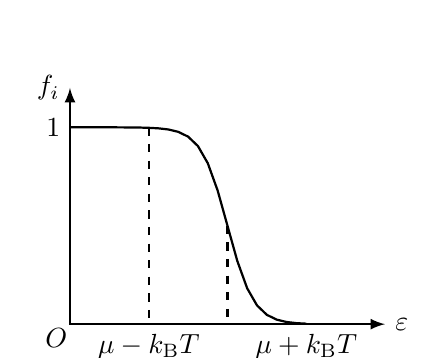
\begin{tikzpicture}
		\coor 43{\varepsilon}{f_i};
		\draw[thick,dashed](2,1.25)--(2,0); % node[below]{$\mu$};
		\draw[thick,dashed](1,2.5)--(1,0)node[below]{$\mu-\kB T$};
		\node[left]at(0,2.5){1};
		\draw[thick,domain=0:3]plot(\x,{2.5/(e^(6*\x-12)+1)})node[below]{$\mu+\kB T$};
	\end{tikzpicture}
	\tikzchap 强简并Fermi气粒子分布
\end{center}
定性估计比热$C_V$:相对$T=0$时,能量增量
\[
	\D E\doteq N\frac{\kB T}{\varepsilon_\Fm}\D\varepsilon,\quad\D\varepsilon=\kB T.
\]
比热
\[
	C_V\doteq 2\kB N\frac{\kB T}{\varepsilon_\Fm}\sim T.
\]

单原子,能量准连续,需计算积分
\[
	Q_\ell:=\int\zti f(\varepsilon)\varepsilon^\ell\d\varepsilon.
\]
注意到$f$的特点,可在$\varepsilon=\mu$展开
\begin{align}\notag
	Q_\ell&=\cancel{\edg{\frac{\varepsilon^\ell}{\ell+1}f(\varepsilon)}\zti}-\frac1{\ell+1}\int\zti f'(\varepsilon)\varepsilon^{\ell+1}\d\varepsilon % =:\int\zti f'(\varepsilon)\upsilon(\varepsilon)
	\d\varepsilon\\
	&=\sum_{n=0}^\infty\frac{\upsilon^{(n)}(\mu)}{n!}\int\zti f'(\varepsilon)(\varepsilon-\mu)^n\d\varepsilon,\quad\upsilon(\varepsilon):=-\frac{\varepsilon^{\ell+1}}{\ell+1}.
\end{align}
令$\eta:=\beta(\varepsilon-\mu)$,则
\[
	f(\varepsilon)=\frac1{\e\eta+1},\quad f'(\varepsilon)=-\frac{\beta\e\eta}{(\e\eta+1)^2}
\]
故
\[
	Q_\ell=-\sum\fmto n0\frac{\upsilon^{(n)}(\mu)}{n!\beta^n}\int_{-\beta\mu}^{+\infty}\frac{\eta^n\e\eta}{(\e\eta+1)^2}\d\eta.
\]

低温下,积分下限$-\beta\mu\to-\infty$
\begin{align*}
	Q_\ell&\doteq-\sum\fmto n0\frac{\upsilon^{(n)}(\mu)}{n!\beta^n}\int\iti\frac{\eta^n\e\eta}{(\e\eta+1)^2}\d\eta\\
	&=-\fkh{\upsilon(\mu)+\frac{\upsilon''(\mu)}{2\beta^2}\frac{\pi^2}3+\cdots}.
\end{align*}
故
\begin{align}
	N=CVQ_{1/2}&=\frac23CV\mu^{3/2}\fkh{1+\frac{\pi^2}8\alpha^{-2}+\bigo\!\kh{\alpha^{-4}}};\\
	U=CVQ_{3/2}&=\frac25CV\mu^{5/2}\fkh{1+\frac{5\pi^2}8\alpha^{-2}+\bigo\!\kh{\alpha^{-4}}}.
\end{align}
其中$\alpha^{-1}(T)=-\frac1{\beta\mu}=\frac{\kB T}{\mu}$。

巨配分函数$\ln\Xi=\frac23\beta U$,压强$p=\frac1\beta\pv{\ln\Xi}V$,
熵
\begin{align}\notag
	S&=\kB\kh{\ln\Xi-\alpha\pv{\ln\Xi}\alpha-\beta\pv{\ln\Xi}\beta}\\\notag
	&=\kB\frac4{15}CV\beta^{-3/2}(-\alpha)^{5/2}\fkh{0+\frac{5\pi^2}4\alpha^{-2}+\bigo\!\kh{\alpha^{-4}}}\\
	&=\frac{\pi^2}3CV\mu^{1/2}\kB^2T\fkh{1+\bigo\!\kh{\alpha^{-2}}}.
\end{align}

利用
\[
	N=\frac23CV\varepsilon_\Fm^{3/2}.
\]
结合$\varepsilon_\Fm=\mu_0$反解出$\mu$
\[
	\mu=\mu_0\fkh{1-\frac{\pi^2}{12}\alpha^{-2}+\bigo\!\kh{\alpha^{-4}}},
\]
不同于Bose气体,$\mu$可正可负。

宏观量用可观测量表示
\begin{gather}
	U=U_0\fkh{1+\frac{5\pi^2}{12}\kh{\frac T{T_\Fm}}^2+\bigo(T^4)},\\
	C_V=N\kB\cdot\frac{\pi^2}{2}\frac T{T_\Fm}\fkh{1+\bigo(T^2)}.\label{CV-Fermi}
\end{gather}
电子气对金属热容量的贡献首先由Sommerfeld解决。

因此低温下金属比热的实验值是电子气和晶格振动(Debye模型)共同贡献
\[
	C_V\sim \underset{\text{Fermi}}{c_\elc T}+\underset{\text{Debye}}{c_\vb T^3}.
\]
与实验符合得很好。
\begin{example}{电子比热vs.晶格比热}{}
	低温下,式 \ref{CV-Debye} 给出晶格比热和式 \ref{CV-Fermi} 给出电子气比热分别为
	\[
	C_V^\vb=N\kB\frac{12\pi^4}5\kh{\frac T{\theta_\Db}}^3,\quad C_V^\elc=N\kB\frac{\pi^2}2\frac T{T_\Fm}.
	\]
	对铜,$\theta_\Db\sim\SI{300}\K,\;T_\Fm\sim\SI{8e4}\K$,二者比值
	\[
	\frac{C_V^\elc}{C_V^\vb}=\frac5{24\pi^2}\frac T{T_\Fm}\kh{\frac{\theta_\Db}T}^3\sim\frac8{T^2}.
	\]
\end{example}
\clearpage
\section{系综}
前面讨论的是近独立粒子系统,忽略粒子间作用,用单粒子态分布描述系统状态;如果粒子间作用不能忽略,单粒子态无确切含义,就要以系统为整体研究,这就是\textbf{系综}。系综的平均值就是统计平均值。
\subsection{系统微观状态的描述与统计系综}
经典理论,粒子状态由广义坐标$q$与广义动量$p$描述,张成$\mu$空间。而系统的微观状态由$\varGamma$空间描述
\begin{definition}{$\varGamma$空间}{Gamma Space}
	$\varGamma$空间是所有粒子广义坐标$q_i$与广义动量$p_i$所张的空间,相体积元
	\begin{align}
		\d\Omega=\prod_{i=1}^f\d q_i\nd p_i,
	\end{align}
	其中$f=N\gamma$为整个系统的自由度。
\end{definition}
量子中,系统微观状态用力学量完全集的量子数描述,由不确定度关系,每个量子态在$\varGamma$空间占据相体积$h^f$。
\begin{definition}{系综}{Ensemble}
	系综(ensemble)是大量微观结构、宏观条件相同的系统的集合。
	\begin{compactitem}
		\item 微正则系综(microcanonical):孤立系统,$N,V,U$恒定;
		\item 正则系综(canonical):\qquad\quad\enspace 封闭系统,$N,V,T$恒定;
		\item 巨正则系综(grand canonical):开放系统,$\mu,V,T$恒定。
	\end{compactitem}
\end{definition}
后面会看到,在粒子数$N\to\infty$且$N/V$恒定时,三个系综等价。
\subsection{微正则分布}
平衡的孤立系统服从的分布叫微正则分布。满足Boltzmann等几率假设:处平衡态的孤立系统,各可能微观状态出现的几率相等。

微正则系综的特性函数就是熵
\[
	\rho_\st=\frac1\Omega,\quad S=-\sum_\st\rho_\st\ln\rho_\st.
\]
\subsection{正则分布}
考虑系统$A$与热源$A_\rs$间的平衡,注意到$A+A_\rs$构成孤立系统,当二者相互作用可忽略时,总能量$E^{(0)}=E_\st+E_\rs$,且对很大的热源$E_\rs\gg E_\st$。记当$A$处于系统$E_\st$某一量子态,$A_\rs$处于系统$E_\rs$任一量子态,微观态数目为$\Omega_\rs(E_\rs)$
\[
	\ln\Omega_\rs(E_\rs)=\ln\Omega_\rs(E^{(0)}-E_\st)\doteq\ln\Omega_\rs(E^{(0)})-\beta E_\st
\]
故分布概率
\[
	\rho_\st\propto\e{-\beta E_\st}\normalize\rho_\st=Z^{-1}\e{-\beta E_\st}.
\]
配分函数
\[
	Z=\sum_\st\e{-\beta E_\st}.
\]
由定义,$\beta$只与热源有关,不同系统达到平衡时温度相同,故$\beta=\beta(T)$。

若能级有简并度$\varGamma_\st$,则 
\begin{align}
	Z=\sum_\st\varGamma_\st\e{-\beta E_\st}.
\end{align}
\paragraph*{正则分布的热力学公式}内能
\begin{align}
	E=\sum_\st\rho_\st E_\st=Z^{-1}\sum_\st E_\st\e{-\beta E_\st}=-\pv{\ln Z}\beta.
\end{align}
物态方程
\begin{align}
	Y_i=\sum_\st\rho_\st\pv{E_\st}{y_i}=-\frac1\beta\pv{\ln Z}{y_i}.
\end{align}
熵
\begin{align*}
	T\d S&=\d E-\sum_i Y_i\d y_i=-\d\kh{\pv{\ln Z}\beta}+\frac1\beta\sum_i\pv{\ln Z}{y_i}\d y_i\\
	&=-\d\kh{\pv{\ln Z}\beta}+\frac1\beta\fkh{\d(\ln Z)-\pv{\ln Z}\beta\d\beta}\\
	&=\frac1\beta\d\kh{\ln Z-\beta\pv{\ln Z}\beta}.
\end{align*}
两边全微分要求$\kB T=\beta$,且 
\begin{align}
	S-S'=\kB\kh{\ln Z-\beta\pv{\ln Z}\beta}=\kB(\ln Z+\beta E).
\end{align}

另一方面,由Boltzmann关系
\begin{align*}
	S&=\kB\ln\Omega\{M_\st\}=\kB\kh{\ln M!-\sum_\st\ln M_\st!}\\
	&\doteq\kB\fkh{M(\ln M-1)-\sum_\st M_\st(\ln M_\st-1)}
\end{align*}
而
\[
	\ln M_\st=\ln M-\ln Z-\beta E_\st
\]
故$S'=0$。

从微观角度说,
\begin{align}
	S=-\kB\sum_\st\rho_\st\ln\rho_\st.
\end{align}
自由能
\begin{align}
	F=E-TS=-\kB T\ln Z.
\end{align}
\paragraph*{能量涨落}由
\begin{align*}
	\ave{E^2}&=\sum_\st\rho_\st E_\st^2=Z^{-1}\sum_\st E_\st^2\e{-\beta E_\st}\\
	&=Z^{-1}\pv[2]Z\beta=\pv[2]{\ln Z}\beta+\kh{\pv{\ln Z}\beta}^2\\
	&=\kB T^2C_V+\ave E^2
\end{align*}
能量的绝对涨落
\begin{align}
	\D E^2=\ave{E^2}-\ave E^2=\kB T^2C_V.
\end{align}
\begin{example}{单原子分子理想气体的相对涨落}{}
	能量$E=\frac32 N\kB T$,比热$C_V=\frac32N\kB$,故相对涨落
	\[
		\vd E=\frac{\D E}E=\sqrt{\frac2{3N}}\sim 10^{-11}
	\]
	涨落对宏观系统量很小的。
\end{example}
因而,$E$可看作是孤立系统的能量,用正则分布研究孤立系统。
\paragraph*{正则分布的连续形式}$\varGamma$空间中,若能量准连续
\begin{align}
	Z=\frac1{N!}\frac1{h^f}\int\e{-\beta E}\prod_{i=1}^N\d q_i\nd p_i
\end{align}
能量曲面$H(p,q,y)=E$包围的相体积
\begin{align}
	\Omega(E)=\int_{H\leqslant E}\prod_{i=1}^N\d q_i\nd p_i.
\end{align}
故按能量分布
\begin{align}
	Z=\frac1{N!}\frac1{h^f}\int\zti\Omega'(E)\e{-\beta E}\d E.
\end{align}
\begin{example}{用正则分布求单原子理想气体物态方程}{}
	$N$个单原子分子气体的Hamilton量
	\[
		H=\sum_{i=1}^{3N}\frac{p_i^2}{2m}.
	\]
	则
	\[
		\Omega(E)=\int\d q\int_{H\leqslant E}\d p=V^N\cdot\frac{\pi^{3N/2}}{\kh{\frac{3N}2}!}(2mE)^{3N/2}.
	\]
	故
	\begin{align*}
		Z&=\frac1{N!h^{3N}}\int\zti\Omega'(E)\e{-\beta E}\d E\\
		&=\frac{V^N}{N!\kh{\frac{3N}2}!}\kh{\frac{2\pi m}{h^2}}^{3N/2}\cdot\frac{3N}2\int\zti E^{3N/2-1}\e{-\beta E}\d E\\
		&%=\frac{V^N}{N!\kh{\frac{3N}2}!}\kh{\frac{2\pi m}{h^2}}^{3N/2}\cdot\frac{3N}2\beta^{-3N/2}\Gamma\kh{\frac{3N}2}
		=\frac{V^N}{N!}\kh{\frac{2\pi m}{h^2\beta}}^{3N/2}=\frac{Z_\tl^N}{N!}.
	\end{align*}
	内能
	\begin{align}
		E=-\pv{\ln Z}\beta=\frac{3N}{2\beta}=\frac32N\kB T.
	\end{align}
	物态方程
	\begin{align}
		p=\frac1\beta\pv{\ln Z}V=\frac N{\beta V}=\frac{N\kB T}V.
	\end{align}
\end{example}
\subsection[实际气体的物态方程]{实际气体(非理想气体)的物态方程}
$N$个全同粒子,体积$V$,
\[
	E=E_\tl+\varPhi+E_\i.
\]
其中$E_\tl(p)$与质心平动有关,$\varPhi(q)$是分子间势能,$E_\i$是分子内部运动。故
\[
	Z=\frac1{N!h^{3N}}\int\e{-\beta E_\tl}\d p\int\e{-\beta\varPhi}\d q\cdot Z_\i.
\]
考虑分子间势能项
\[
	Q:=\int\e{-\beta\varPhi}\d q
\]
只考虑分子间两两相互作用,其作用势$\phi_{ij}\equiv\phi(r_{ij})$只与分子间距离有关,
\[
	\varPhi=\sum_{i<j}\phi_{ij}
\]
引入
\[
	f_{ij}=\e{-\beta\phi_{ij}}-1=
	\begin{cases}
		0,&r_{ij}\to\infty\\
		-1,&r_{ij}\to0
	\end{cases}
\]
分子作用力是短程的,故一般$\abs{f_{ij}}<1$,可展开
\[
	Q=\int\prod_{i<j}(1+f_{ij})\d q=\int\fkh{1+\sum_{i<j}f_{ij}+\frac12\overset{(i,j)\neq(k,\ell)}{\sum_{i<j}\sum_{k<\ell}}f_{ij}f_{k\ell}+\cdots}\d q.
\]
第三项后仅当多个分子都很接近时才显著,故只保留前两项
\[
	Q\doteq V^N+\frac12N(N-1)V^{N-2}\int f(r_{12})\d\bm r_1\nd\bm r_2.
\]
引入质心坐标$\bm R=\frac{m_1\bm r_1+m_2\bm r_2}{m_1+m_2}$和相对位置$\bm r=\bm r_1-\bm r_2$,易证$\det J=1$
\[
	\int f(r_{12})\d\bm r_1\nd\bm r_2=\int f(r)\d\bm r\nd\bm R=-2Va_2(T).
\]
第二级Virial系数
\begin{align}
	a_2(T)=-\frac12\int f(r)\d\bm r=-2\pi\int\zti\kh{\e{-\beta\phi(r)}-1}r^2\d r
\end{align}
故
\[
	Q\doteq V^N-N(N-1)V^{N-1}a_2(T)\doteq V^N\fkh{1-\frac{N^2}Va_2(T)}.
\]
取对数\footnote{过程中一系列近似相当于
\[
	\ln\e{-x}=\ln\kh{1-x+\frac12x^2+\cdots}\doteq\ln(1-x)\doteq -x
\]
即结果并不会不严格。}
\begin{align}
	\ln Q=N\ln V+\ln\fkh{1-\frac{N^2}Va_2(T)}\doteq N\ln V-\frac{N^2}Va_2(T).
\end{align}
物态方程
\begin{align*}
	p=\frac1\beta\pv{\ln Q}V=\frac1\beta\fkh{\frac NV+\frac{N^2}{V^2}a_2(T)}.
\end{align*}
故
\begin{align}
	\frac{pv}{\kB T}=1+\frac{a_2(T)}v.
\end{align}
\begin{example}{Van der Waals力}{Van der Waals Force}
	1930年London证明瞬时电偶极矩之间力
	\begin{center}
		\(\phi(r)=\phi_0\fkh{\kh{\frac{r_0}r}^{12}-2\kh{\frac{r_0}r}^6}\doteq\begin{cases}
			\infty,&r<r_0\\
			-\phi_0\kh{\frac{r_0}r}^6,&r>r_0
		\end{cases}\)

		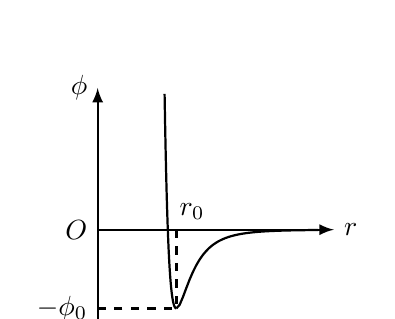
\begin{tikzpicture}
			\draw[thick,-latex](0,0)node[left]{$O$}--(3,0)node[right]{$r$};
			\draw[thick,-latex](0,-1.2)--(0,1.8)node[left]{$\phi$};
			\draw[thick,dashed](1,0)--(1,-1)--(0,-1)node[left]{$-\phi_0$};
			\node[above]at(1.2,0){$r_0$};
			\draw[thick,domain=.85:1]plot(\x,{\x^(-12)-2*\x^(-6)});
			\draw[thick,domain=1:2]plot(\x,{\x^(-12)-2*\x^(-6)});
			\draw[thick,domain=2:2.8]plot(\x,{\x^(-12)-2*\x^(-6)});
		\end{tikzpicture}
		\tikzchap $\phi\vs r$图像
	\end{center}
	故
	{\begin{align*}
		a_2(T)&=-2\pi\int_0^{r_0}-r^2\d r-2\pi\int_{r_0}^{+\infty}\fkh{\e{-\beta\phi(r)}-1}r^2\d r\\
		&\doteq\frac{2\pi}3r_0^3+2\pi\int_{r_0}^{+\infty}\beta\phi(r)r^2\d r\tag{$\kB T\gg\phi_0$}\\
		&=\frac{2\pi}3r_0^3-\frac{2\pi}3\frac{\phi_0r_0^3}{\kB T}=:b-\frac a{\kB T}.
	\end{align*}}
	又$b=4v_0\ll v$
	\[
		\frac{pv}{\kB T}=1+\frac bv-\frac a{v\kB T}\doteq\frac1{1-b/v}-\frac a{v\kB T}.
	\]
	故Van der Waals方程
	\begin{align}
		\kh{p+\frac a{v^2}}(v-b)=\kB T.
	\end{align}
\end{example}
\subsection{Ising模型}
对于Fe, Ni, Co等铁磁性物质,存在Curie温度$T_\Cr$,当$T<T_\Cr$时会有自发磁化现象,而$T>T_\Cr$时消磁。1920年Lenz为解释铁磁-顺磁相变提出一个模型,并由其学生Ising求解出一维的情形(一维模型无相变)。

\paragraph*{Ising模型}$N$个取值为$\pm 1$($\uparrow\downarrow$)的格点$S_i$,系统的能量包括邻对的相互作用和外磁场能
\begin{align}
	E\{S_i\}=-\sum_{ij}\varepsilon_{ij}S_iS_j-\mu_0\mu H\sum_iS_i
\end{align}
对于各向同性的物质$\varepsilon_{ij}=\varepsilon$
\[
	E\{S_i\}=-\varepsilon\sum_{ij}S_iS_j-\mu_0\mu H\sum_iS_i.
\]
配分函数
\[
	Z=\prod_{i=1}^N\sum_{S_i=\pm 1}\e{-\beta E\{S_i\}}.\]
\paragraph*{平均场近似}作用于$S_i$的力为 
\[
	-\pv E{S_i}=\sum_j\varepsilon_{ij}S_j+\mu_0\mu H.
\]
可视为等效外场
\[
	H_i=H+\frac1{\mu_0\mu}\sum_j\varepsilon_{ij}S_j.
\]
其平均值
\[
	\avg H=H+\frac1{\mu_0\mu}z\varepsilon\avg S,
\]
其中$z$为任一给定格点的最近邻格点数,对于二维方阵,$z=4$。
\clearpage
用平均场$\avg H$代替外场$H$并忽略其涨落,这样相互作用自旋系统便化为近独立的自旋系统,配分函数
\[
	Z=\prod_{i=1}^N\sum_{S_i=\pm 1}\e{\beta\mu_0\mu\avg H S_i}=\kh{\e{\beta\mu_0\mu\avg H}+\e{-\beta\mu_0\mu\avg H}}^N.
\]
磁矩
\begin{align}
	M=\frac1\beta\pv{\ln Z}{\mu_0 H}=N\mu\tanh\beta\mu_0\mu\avg H.
\end{align}

不加外场时$H=0$,有
\begin{align}
	M=N\mu\avg S=N\mu\tanh\beta z\varepsilon\avg S.\thus\avg S=\tanh\beta z\varepsilon\avg S.
\end{align}
由$y=\tanh x$图像的性质,当$\beta z\varepsilon\leqslant 1$时,只有$\avg S=0$的解,自发磁化为0,顺磁态;而当$\beta z\varepsilon>1$时,有非零的自发磁化,铁磁态。相变的临界温度
\begin{align}
	T_\Cr=\frac{z\varepsilon}\kB.
\end{align}
Ising模型在平均场近似下的临界指数与Landau模型相同,详见作业。
\subsection{巨正则分布}
%巨正则分布是$V$恒定,并与恒温粒子源接触而达平衡系统服从的分布,平衡时,温度$T$和化学势$\mu$相同。

与正则分布相似,系统与热源构成孤立系统,总能量和总粒子数恒定。系统处于处粒子数为$N$,能量为$E_\st$的某一量子态的几率
\[
	\rho_{N\st}\propto\Omega_\rs(N_\rs,E_\rs)=\Omega_\rs(N^{(0)}-N,E^{(0)}-E_\st).
\]
$N^{(0)}\gg N,E^{(0)}\gg E_\st$,故可在$(N^{(0)},E^{(0)})$处展开
\[
	\ln\Omega_\rs(N^{(0)}-N,E^{(0)}-E_\st)\doteq\ln\Omega_\rs(N^{(0)},E^{(0)})-\alpha N-\beta E_\st.
\]
其中$\alpha=\alpha(T,\mu),\;\beta=\beta(T)$只与热源有关,故
\begin{align}
	\rho_{N\st}=\Xi^{-1}\e{-\alpha N-\beta E_\st}.
\end{align}
其中巨配分函数
\begin{align}
	\Xi=\sum_{N=0}^\infty\sum_\st\e{-\alpha N-\beta E_\st}.
\end{align}
\paragraph*{连续形式}对不同粒子数$N$,需定义不同维数的$\Gamma$空间,设粒子自由度为$r$,则系统自由度为$f=Nr$:
\begin{align}
	\Xi=\sum_{N=0}^\infty\frac1{N!h^{Nr}}\e{-\alpha N}\int\e{-\beta E(q,p,y)}\prod_{i=1}^N\d q_i\nd p_i.
\end{align}
\paragraph*{巨配分函数与配分函数的关系}有时,如量子统计情形,$\Xi$比$Z$计算方便
\[
	\Xi(\alpha,\beta,y)=\sum_{N=0}^\infty\sum_\st\e{-\alpha N-\beta E_\st}=\sum_Nq^NZ_N(\beta,y).
\]
其中易逸度(Fugacity) $q=\e{-\alpha}$

\paragraph*{巨正则分布的热力学公式}宏观量等于对应微观量的统计平均值
\begin{align}
	\avg N=\sum_N\sum_\st N\rho_{N\st}=-\pv{\ln\Xi}\alpha.
\end{align}
内能
\begin{align}
	U=\avg E=\sum_N\sum_\st E_\st\rho_{N\st}=-\pv{\ln\Xi}\beta.
\end{align}
物态方程
\begin{align}
	\avg Y=\sum_N\sum_\st\pv{E_\st}y\rho_{N\st}=-\frac1\beta\pv{\ln\Xi}y.
\end{align}
熵,首先由
\begin{align*}
	\d\kh{\ln\Xi+\alpha\avg N+\beta\avg E}=\alpha\d\avg N+\beta\d\avg E-\beta\avg Y\d y=\beta\kh{\d\avg E-\avg Y\d y+\frac\alpha\beta\d\avg N}.
\end{align*}
故$\mu=-\frac\alpha\beta,\;\beta=\frac1{\kB T}$,熵
\begin{align}
	S=\kB\kh{\ln\Xi+\alpha\avg N+\beta\avg E}{\color{lightgray}\,+\,S'}.
\end{align}
由Boltzmann关系,$S'=0$
\begin{align}
	S=-\kB\sum_N\sum_\st\rho_{N\st}\ln\rho_{N\st}.
\end{align}
\paragraph*{巨正则势}
由熵的表达式知,
\[
	\ln\Xi=\frac{ST+\mu\avg N-\avg E}{\kB T}=\frac{pV}{\kB T}.
\]
可定义巨正则势
\begin{align}
	J(T,V,\mu):=-pV=-\kB T\ln\Xi.
\end{align}
有
\[
	\d J=-S\d T-p\d V-N\d\mu.
\]
\paragraph*{涨落}
粒子数涨落
\begin{align}
	\D N^2=\ave{N^2}-\ave N^2=-\pv{\avg N}\alpha=\kB T\kh{\pv{\avg N}\mu}_{T,V}.
\end{align}
能量涨落
\begin{align}
	\D E^2=\kB T^2C_V+\kh{\pv EN}_{V,T}^2\D N^2.
\end{align}
\paragraph*{由巨正则分布导出近独立粒子系统的平衡分布}系统处粒子数$N$,能量$E_\st$的几率
\[
	\rho_{Na}=\Xi^{-1}\Omega_\st\e{-\alpha N-\beta E_\st}.
\]
其中$\Omega_\st$为$E_\st$的简并度。

对于近独立粒子系统,单粒子能级$\varepsilon_i$,简并度$\omega_i$,对应分布$\{a_i\}$时,系统粒子数$N_{\{a_i\}}$,能量$E_{\{a_i\}}$
\[
	N_{\{a_i\}}=\sum_ia_i,\quad E_{\{a_i\}}=\sum_ia_i\varepsilon_i.
\]
微观态数
\[
	\Omega_{\{a_i\}}=\prod_i\Omega_{a_i}.
\]
其中$\Omega_{a_i}$为$a_i$个粒子在$\varepsilon_i$能级上微观方式数。

系统具有分布$\{a_i\}$的几率:
\[
	\rho_{\{a_i\}}=\Xi^{-1}\Omega_{\{a_i\}}\e{-\alpha N_{\{a_i\}}-\beta E_{\{a_i\}}}=\Xi^{-1}\prod_i\Omega_{a_i}\e{-\alpha{a_i}-\beta{a_i\varepsilon_i}}.
\]
总巨配分函数
\[
	\Xi=\sum_{\{a_i\}}\prod_i\Omega_{a_i}\e{-\alpha{a_i}-\beta{a_i\varepsilon_i}}=\prod_i\Xi_i.
\]
其中 
\[
	\Xi_i=\sum_{a_i}\Omega_{a_i}\e{-\alpha{a_i}-\beta{a_i\varepsilon_i}}.
\]
则
\begin{align*}
	\avg{a_i}=\sum_{\{a_i\}}a_i\rho_{\{a_i\}}=\Xi_i^{-1}\sum_{a_i}a_i\Omega_{a_i}\e{-\alpha{a_i}-\beta{a_i\varepsilon_i}}=-\pv{\ln\Xi_i}\alpha.
\end{align*}

Bose分布
\begin{align}
	\Omega_{a_i}=\binom{a_i+\omega_i-1}{a_i}=\frac{(a_i+\omega_i-1)!}{a_i!(\omega_i-1)!}.
\end{align}
则由$(1+x)^{-n}$的Taylor展开
\begin{align}
	\Xi_i&=\sum_{a_i=0}^\infty\frac{(a_i+\omega_i-1)!}{a_i!(\omega_i-1)!}\e{-\alpha a_i-\beta a_i\varepsilon_i}=\kh{1-\e{-\alpha-\beta\varepsilon_i}}^{-\omega_i};\\
	a_i&=-\pv{\ln\Xi_i}\alpha=\frac{\omega_i}{\e{\alpha+\beta\varepsilon_i}-1}.
\end{align}

Fermi分布
\begin{align}
	\Omega_{a_i}=\binom{\omega_i}{a_i}=\frac{\omega_i!}{a_i!(\omega_i-a_i)!}.
\end{align}
由$(1+x)^n$的二项式展开
\begin{align}
	\Xi_i&=\sum_{a_i=0}^{\omega_i}\frac{\omega_i!}{a_i!(\omega_i-a_i)!}\e{-\alpha a_i-\beta a_i\varepsilon_i}=\kh{1+\e{-\alpha-\beta\varepsilon_i}}^{-\omega_i};\\
	a_i&=-\pv{\ln\Xi_i}\alpha=\frac{\omega_i}{\e{\alpha+\beta\varepsilon_i}+1}.
\end{align}
这也正是巨配分函数的由来。

半经典分布$\omega_i\gg a_i$ 
\begin{align}
	\Omega_{a_i}=\frac{\omega_i^{a_i}}{a_i!}.
\end{align}
由$\e{x}$的Taylor展开
\begin{align}
	\Xi_i&=\sum_{a_i=0}^\infty\frac{\omega_i^{a_i}}{a_i!}\e{-\alpha a_i-\beta a_i\varepsilon_i}=\e{\omega_i\e{-\alpha-\beta\varepsilon_i}};\\
	a_i&=-\pv{\ln\Xi_i}\alpha=\omega_i\e{-\alpha-\beta\varepsilon_i}.
\end{align}
\clearpage
\section{非平衡态统计理论初步}
平衡态性质及其统计方法存在大量非平衡态和不可逆过程。本章主要讨论稀薄气体的非平衡性质分子运动论方法。
\subsection{气体分子的碰撞频率}
气体分子通过碰撞使气体达致平衡。
单位时间内碰到单位面积器壁上的分子数$\Gamma$,定义分布函数$f(\bm r,\bm v,t)$,则
\[
	\Gamma(\bm r,t)=\int f(\bm r,\bm v,t)v_x\d\bm v.
\]
若为平衡态,则满足Maxwell分布$\Gamma=n\avg v/4$。

采用弹性刚球模型(无摩擦,无形变,弹性碰撞)。对于稀薄气体,只考虑两体碰撞,对于两类不同分子间碰撞:单位时间内,平均一个分子1与分子2的碰撞次数$\theta_{12}$,称碰撞频率。

指定速度的分子1的碰撞:
单位时间内,一个速度$v_1$的分子1与任意速度的分子2碰撞次数$\theta_{12}(\bm r,\bm v_1,t)$。碰撞只与相对速度$\bm g_{21}=\bm v_2-\bm v_1$有关。发生碰撞的有效截面积$\pi\sigma^2_{12}$,其中$\sigma_{12}=(\sigma_1+\sigma_2)/2$为两分子直径平均值。易知,这个条件是各向同性的。
\begin{align}
	\theta_{12}(\bm r,\bm v_1,t)=\pi\sigma_{12}^2\Gamma=\pi\sigma_{12}^2\int f_2(\bm r,\bm v_2,t)g_{12}\d\bm v_2,
\end{align}
以上采用了分子混沌假设,即分子速度分布是独立的:
\[
	f(\bm r,\bm v_1,\bm v_2,t)\doteq f_1(\bm r,\bm v_1,t)f_2(\bm r,\bm v_2,t).
\]

故单位时间内,平均一个分子1与分子2碰撞次数
\begin{align}
	\theta_{12}(\bm r,t)=\frac1{n_1(\bm r_1,t)}\int f_1(\bm r,\bm v_1,t)\theta_{12}(\bm r,\bm v_1,t)\d\bm v_1.
\end{align}
\paragraph*{两体碰撞运动学}
弹性碰撞满足动量守恒和能量守恒
\begin{align}
	m_1\bm v_1+m_2\bm v_2&=m_1\bm v_1'+m_2\bm v_2'\\
	\frac12m_1v_1^2+\frac12m_2v_2^2&=\frac12m_1{v'_1}^2+\frac12m_2{v'_2}^2.
\end{align}
4方程,6未知数,需指定碰撞方向$\bm n$ (或散射角$\theta,\phi$)才能完全决定末态速度。

设速度改变方向$\bm n$,即
\begin{gather*}
	(m_1,\bm v_1)+(m_2,\bm v_2)\quad\overset{\bm n}{\longrightarrow}\quad(m_1,\bm v_1')+(m_2,\bm v_2').\\
	\bm v_1'-\bm v_1=\lambda_1\bm n,\quad\bm v_2'-\bm v_2=\lambda_2\bm n.
\end{gather*}
带入守恒方程
\begin{align*}
	\begin{cases}
		m_1\lambda_1+m_2\lambda_2=0,\\
		m_1\lambda_1(\bm v_1+\bm v_1')\cdot\bm n+m_2\lambda_2(\bm v_2+\bm v_2')\cdot\bm n=0.
	\end{cases}
\end{align*}
解出$\lambda_1,\lambda_2$,
\begin{align}
	\begin{cases}
		\bm v_1'=\bm v_1+\frac{2m_1}{m_1+m_2}\zkh{(\bm v_2-\bm v_1)\cdot\bm n}\bm n\\[1ex]
		\bm v_2'=\bm v_2+\frac{2m_2}{m_1+m_2}\zkh{(\bm v_1-\bm v_2)\cdot\bm n}\bm n
	\end{cases}
\end{align}
对称性:
\begin{compactenum}
	\item 碰撞前后相对速度不变
	\[
		\bm v_1'-\bm v_2'=\bm v_1-\bm v_2-2\zkh{(\bm v_1-\bm v_2)\cdot\bm n}\bm n\thus g_{21}'=g_{21}.
	\]
	\item 碰撞前后相对速度沿碰撞方向变号,垂直方向不变
	\begin{align*}
		(\bm v_1'-\bm v_2')\cdot\bm n&=-(\bm v_1-\bm v_2)\cdot\bm n,\\
		(\bm v_1'-\bm v_2')\times\bm n&=(\bm v_1-\bm v_2)\times\bm n.
	\end{align*}
	\item 原碰撞与逆碰撞等价。所谓逆碰撞:
	\[
		(m_1,\bm v_1')+(m_2,\bm v_2')\quad\overset{-\bm n}{\longrightarrow}\quad(m_1,\bm v_1)+(m_2,\bm v_2).
	\]
\end{compactenum}
\subsection{Boltzmann输运方程}
讨论分布函数如何随时间变化,记$t$时刻,$(\bm r,\bm v)$处体积元在$\mu$空间$\d\bm r\nd\bm v$中的分子数$f(\bm r,\bm v,t)\d\bm r\nd\bm v$。

将分子作为经典粒子处理,故只适用于高温情形
\[
	\lambda_T=\kh{\frac{h^2}{2\pi m\kB T}}^{3/2}\ll\kh{\frac VN}^{1/3}.
\]
稀薄气体近似: 分子除碰撞短时间隔处是自由的。(高温低密度)

因此$\p f/\p t$可看成两部分贡献:漂移项(drift)和碰撞项(collision)
\begin{align}
	\pv ft=\kh{\pv ft}_\df+\kh{\pv ft}_\cll.
\end{align}
漂移项代表运动使$\bm r$变化,外场使$\bm v$变化;碰撞项代表碰撞使$\bm v$变化。
\paragraph*{漂移项}首先考虑位置变化:$\d t$内,由$x$处垂直$x$轴的平面进入,和由$x+\d x$处垂直$x$轴的平面离开体积元的分子数所产生的净增加分子数
\[
	\fkh{f(x,y,\ldots)-f(x+\d x,y,\ldots)}\d y\nd z\nd\bm v\cdot v_x\d t=-v_x\pv fx\d\bm r\nd\bm v\d t.
\]
计所有分量
\[
	-\bm v\cdot\nabla_{\bm r}f(\bm r,\bm v,t)\d\bm r\nd\bm v\nd t.
\]

类似的,$x$方向速度变化所产生的净增加分子数
\[
	-\pp{v_x}(a_xf)\d\bm r\nd\bm v\nd t\thus-\nabla_{\bm v}(\bm af)\d\bm r\nd\bm v\nd t.
\]
假设作用力与速度$\bm v$无关,则$\bm a$项可提出来,继而
\begin{align}
	\kh{\pv ft}_\df=-\bm v\cdot\nabla_{\bm r}f-\bm a\cdot\nabla_{\bm v}f.
\end{align}
\paragraph*{碰撞项}$\d\bm r\nd\bm v$中分子与别的分子碰撞后离开体积元,称原碰撞,别的分子碰后进入该体积元,称逆碰撞。

原碰撞:$\d t$内,$\d\bm r\nd\bm v$中分子与速度$\bm v_1\to\bm v_1+\d\bm v_1$分子碰撞使分子数减少
\[
	f(\bm r,\bm v,t)\d\bm r\nd\bm v\cdot f(\bm r_1,\bm v_1,t)\d\bm v_1\sigma^2\d\Omega\cdot g\d t\cos\theta=f\!f_1\Lambda\d t\nd\Omega\nd\bm r\nd\bm v\nd\bm v_1.
\]
其中$\Lambda:=\abs{\bm v-\bm v_1}\sigma^2\cos\theta$,相应的逆碰撞
\[
	f'\!f_1'\Lambda\d t\nd\Omega\nd\bm r\nd\bm v\nd\bm v_1.
\]
积分之
\begin{align}
	\kh{\pv ft}_\cll=\intt(f'\!f_1'-f\!f_1)\Lambda\d\Omega\nd\bm v_1.\quad\theta\in\fkh{0,\frac\pi{2}}.
\end{align}
得到Boltzmann输运方程
\begin{align}
	\pv ft+(\bm v\cdot\nabla_{\bm r}+\bm a\cdot\nabla_{\bm v})f=\intt(f'\!f_1'-f\!f_1)\Lambda\d\Omega\nd\bm v_1.
\end{align}
方程左边的项即$\d f/\nd t$,这是一个非线性积分-微分方程,一般难求解。

分子混沌假设对稀薄气体是精确的,但使得Boltzmann方程不封闭,为了求单粒子分布函数$f(\bm r,\bm v,t)$,需先求出两粒子关联函数$f(\bm r,\bm v,\bm v_1,t)$。为求$N-1$粒子关联函数,要先求出$N$粒子关联函数\footnote{BBGKY: Hierarchy, Bogoliubov-Born-Green-Kirkwood-Yvon.},如何截断该方程见Huang \S 3.5。
\subsection{Boltzmann \textit{H}定理}
讨论系统趋向平衡态时,分布函数的性质。定义:$H$函数为分布函数$f(\bm r,\bm v,t)$的泛函
\begin{align}
	H(t)=\int f(\bm r,\bm v,t)\ln f(\bm r,\bm v,t)\d\bm r\nd\bm v.
\end{align}
\begin{theorem}{Boltzmann $H$定理}{Boltzmann H Theorem}
	若$f(\bm r,\bm v,t)$满足Boltzmann输运方程,则
	\begin{align}
		\dv Ht\leqslant 0.
	\end{align}
	当且仅当$f\!f_1=f'\!f_1'$时取等号。
\end{theorem}
\prf 
\begin{align*}
	\dv Ht=\int(1+\ln f)\pv ft\d\bm r\nd\bm v
\end{align*}
漂移项贡献为0
\begin{align*}
	&-\int(1+\ln f)(\bm v\cdot\nabla_{\bm r}f+\bm a\cdot\nabla_{\bm v}f)\d\bm r\nd\bm v\\
	=&-\int\bm v\cdot\nabla_{\bm r}(f\ln f)+\nabla_{\bm v}\cdot(\bm af\ln f)\d\bm r\nd\bm v\tag{Gauss}\\
	=&-\int\bs5\oint \bm v f\ln f\cdot\d\bm S\nd\bm v-\int\bs5\oint\bm af\ln f\cdot\d\bm S_{\bm v}\nd\bm r=0.
\end{align*}
碰撞项贡献
\begin{align*}
	\int (1+\ln f)(f'\!f_1'-f\!f_1)\Lambda\d\Omega\nd\bm v_1\nd\bm r\nd\bm v
\end{align*}
交换$\bm v,\bm v_1$,得到的新式与原式相加除2
\[
	=\frac12\int (2+\ln f\!f_1)(f'\!f_1'-f\!f_1)\Lambda\d\Omega\nd\bm v_1\nd\bm r\nd\bm v
\]
又原逆碰撞对称,交换$\bm v,\bm v'$和$\bm v_1,\bm v_1'$,得到
\[
	=\frac12\int (2+\ln f'\!f_1')(f\!f_1-f'\!f_1')\Lambda\d\Omega\nd\bm v_1\nd\bm r\nd\bm v
\]
二者相加除2,得到
\begin{align}
	\dv Ht=-\frac14\int (\ln f'\!f_1'-\ln f\!f_1)(f'\!f_1'-f\!f_1)\Lambda\d\Omega\nd\bm v_1\nd\bm r\nd\bm v\leqslant 0.
\end{align}
当且仅当$f\!f_1=f'\!f_1'$时取等号。

\paragraph*{讨论}
\begin{compactenum}
	\item 碰撞使$f$改变,从而使$H$不断减小,当$H$达到极小值时,达到平衡态。从统计理论上说明了趋向平衡的不可逆性($H$单调减)。
	\item 可以证明,熵与$H$函数的关系为
	\begin{align}
		S=-\kB H+\cns.
	\end{align}
	因此,$H$趋于极小与$S$趋于极大一致,$H$定理与$S$增原理相当,但有不同之处:
		\subitem $\bullet$ 对任意态可定义$H$,但热力学中$S$仅对平衡态有定义\footnote{可通过Boltzmann关系推广$S$定义。};
		\subitem $\bullet$ 熵增原理适用于任意孤立系,$H$定理前提:$f$满足Boltzmann输运方程,即分子混沌假设成立;
		\subitem $\bullet$ $H$定理给出了系统趋向平衡态的速度,熵增原理不能。
	\item $H$定理具有统计特征,对统计性的$f$再取了一次平均:
	\[
		\dv Ht=N\avg{\ln f}.
	\]
	$H$随时间改变也是统计性的,且不连续,因碰撞而迅速改变。因此$\d H/\nd t$实际上是$\D H/\D t$。
	\item 微观可逆性与宏观不可逆性:当Hamiltion量是动量偶函数时,微观运动中是可逆的。但$H$函数由微观分布决定,却是时间的单调函数。\footnote{Boltzmann指出:$H$定理是统计性的,即平均来说,$H$减少的几率最大,但不排除增大的可能性,只是几率非常小而已,即宏观不可逆性是统计性的,$H$定理不是力学规律,而是统计性的。}	
	\item 微观运动可复原性问题
	
	Poincare定理:有限能量,有限范围的系统,经过足够长时间后,总能回到与初始状态无限接近的状态,称Poincare循环。

	Boltzmann提出:Poincare周期很长,远超出实际观测的时间,因此,在观测时间里,回到原状的几率很小。不同的理解:如Huang \S 4.1, \S 4.4, \S 4.5。
\end{compactenum}
\end{document}